\chapter{Test and Validation of the Proposed Solution}

\renewcommand{\chaptername}{Chapter}

\section*{Introduction}
%After the development conducted in the previous chapter, the results of the implementation 
%and concrete tests are highlighted and discussed.
%This part outlines:
%
%* the initial conditions of the test: Coordiantes of the robot, and the coordinates of the station 
%and its configuration and constraints. and the test scenarios.
%* the results of path planning of the pattern path. 
%* results of the evaluation approach 
%* results of the path optimization
%* Analysis of the Metaheuristics
%* Comparison to OMPL
%* the robot following the generated path. Screenshots of the robot at 3 intermediate positions and mention 
%the coordinates. the robot in its final position.

This chapter presents the results of testing and validating our proposed path planning and optimization algorithms. 
We conducted experiments under various conditions, evaluating factors such as path quality, algorithm 
performance, and robot execution. By comparing our approach to OMPL and analyzing the results, we aim 
to demonstrate the effectiveness of our solution for real-world AMR applications.
For this section 3 test environments are used:
\begin{itemize}
    \item Independent Simulation Environment: This environment is created outside the RACK 
    environment to validate the chosen approaches before implementing the developed features 
    on the real system. It recreates the Station and the Shelf without sensor inputs or kinematic constraints.
    To simplify the test, the robot is modeled by a point instead of its proportional chassis size.

    \item RACK simulation environment: It is the simulation environment used in the team to simulate 
    the outcomes of the developed features in the same conditions as the real test. It includes all the sensor 
    input and makes it available for the test: Localization, Obstacle Detection, and Object Recognition features.
    It can be Offline or Online
    \begin{itemize}
        \item Offline Testing: is the re-creation of the warehouse and the test environment in a complete model
        as seen on figure \Ref{warehouse}. A simulated robot is available to place at a starting point, 
        to navigate the planned paths as well
        as to perceive its surroundings and use the sensor input for its processing. Objects like simulated 
        obstacles can be added. 
        \item Online Testing: is a projection of the test on the AMR to the Simulation environment.
        The simulation visualizes the output of the sensors like scan points and makes a debugging 
        tool available for interpretation of results, debugging, and optimization.
    \end{itemize}

    \item AMR Field Tests: the AMR is commissioned with the test algorithms, validated through the RACK simulation
    environment tests. The truck navigates the planned paths in the real warehouse and deals with real stations, 
    shelves, pallets, obstacles and general surrounding objects.
\end{itemize}

\section{Path Creation Test Results and Validation}
The implemented Path Creation Approach explained in section 3.2.3 was first tested in a simulation environment
composed of one Station. This environment emulates the RACK model of the test warehouse and was used to test 
and validate the approach before testing it inside the RACK simulation first and then on the AMR.

For this environment, the implementation results of the subpolygons from section 3.1 were used for the path creation.
The created subpolygons are used as transition zones. 
As a first test of pure path creation, the transition points are previously fixed at the center of the 
subpolygons. The path is created by placing the robot in the simulation in a starting position and testing 
different target locations.

The obtained results are of smooth splines adhering to the pattern and linking the truck to the destination pallet 
while passing by a transition location. 
The independent Simulation Environment tests show the pattern spline-based path as given by figure \Ref{Test_clone}:
The path start at the truck's position, transitions in one of the transition subpolygons to change driving 
direction and joins the target. 
The resulting path on the RACK simulation environment which is the real testing environment show as well 
the creation and plotting of the pattern path on the simulated station as given by \Ref{TestResults} and \Ref{Test_Simu}.

This approach is validated and is ready as a basis for the next test steps. 
The validation is for the following reasons:
\begin{itemize}
    \item The path creation module integrates the subpoygon functionality successfully: the use of a transition
    point from the subpolygons is effective when tested with a complete path.
    \item The created paths satisfy the intended pattern: they link the truck to the transition point, then, 
    the latter to the target. Inside the RACK simulation environment, it was verified that the direction 
    change occurs: the AMR switches from a negative speed at the first section when driving in opposite 
    direction the first part of the spline path until the transition point, to a positive speed when driving in 
    main driving direction the second part of the spline path from the transition point to the target.
    \item The paths link the start to the chosen target accurately which reflects the validation of the 
    transformations implemented at the development section of the Path Creation.
\end{itemize}

\begin{figure}[H]
    \centering
    \begin{minipage}{0.45\textwidth}
        \centering
        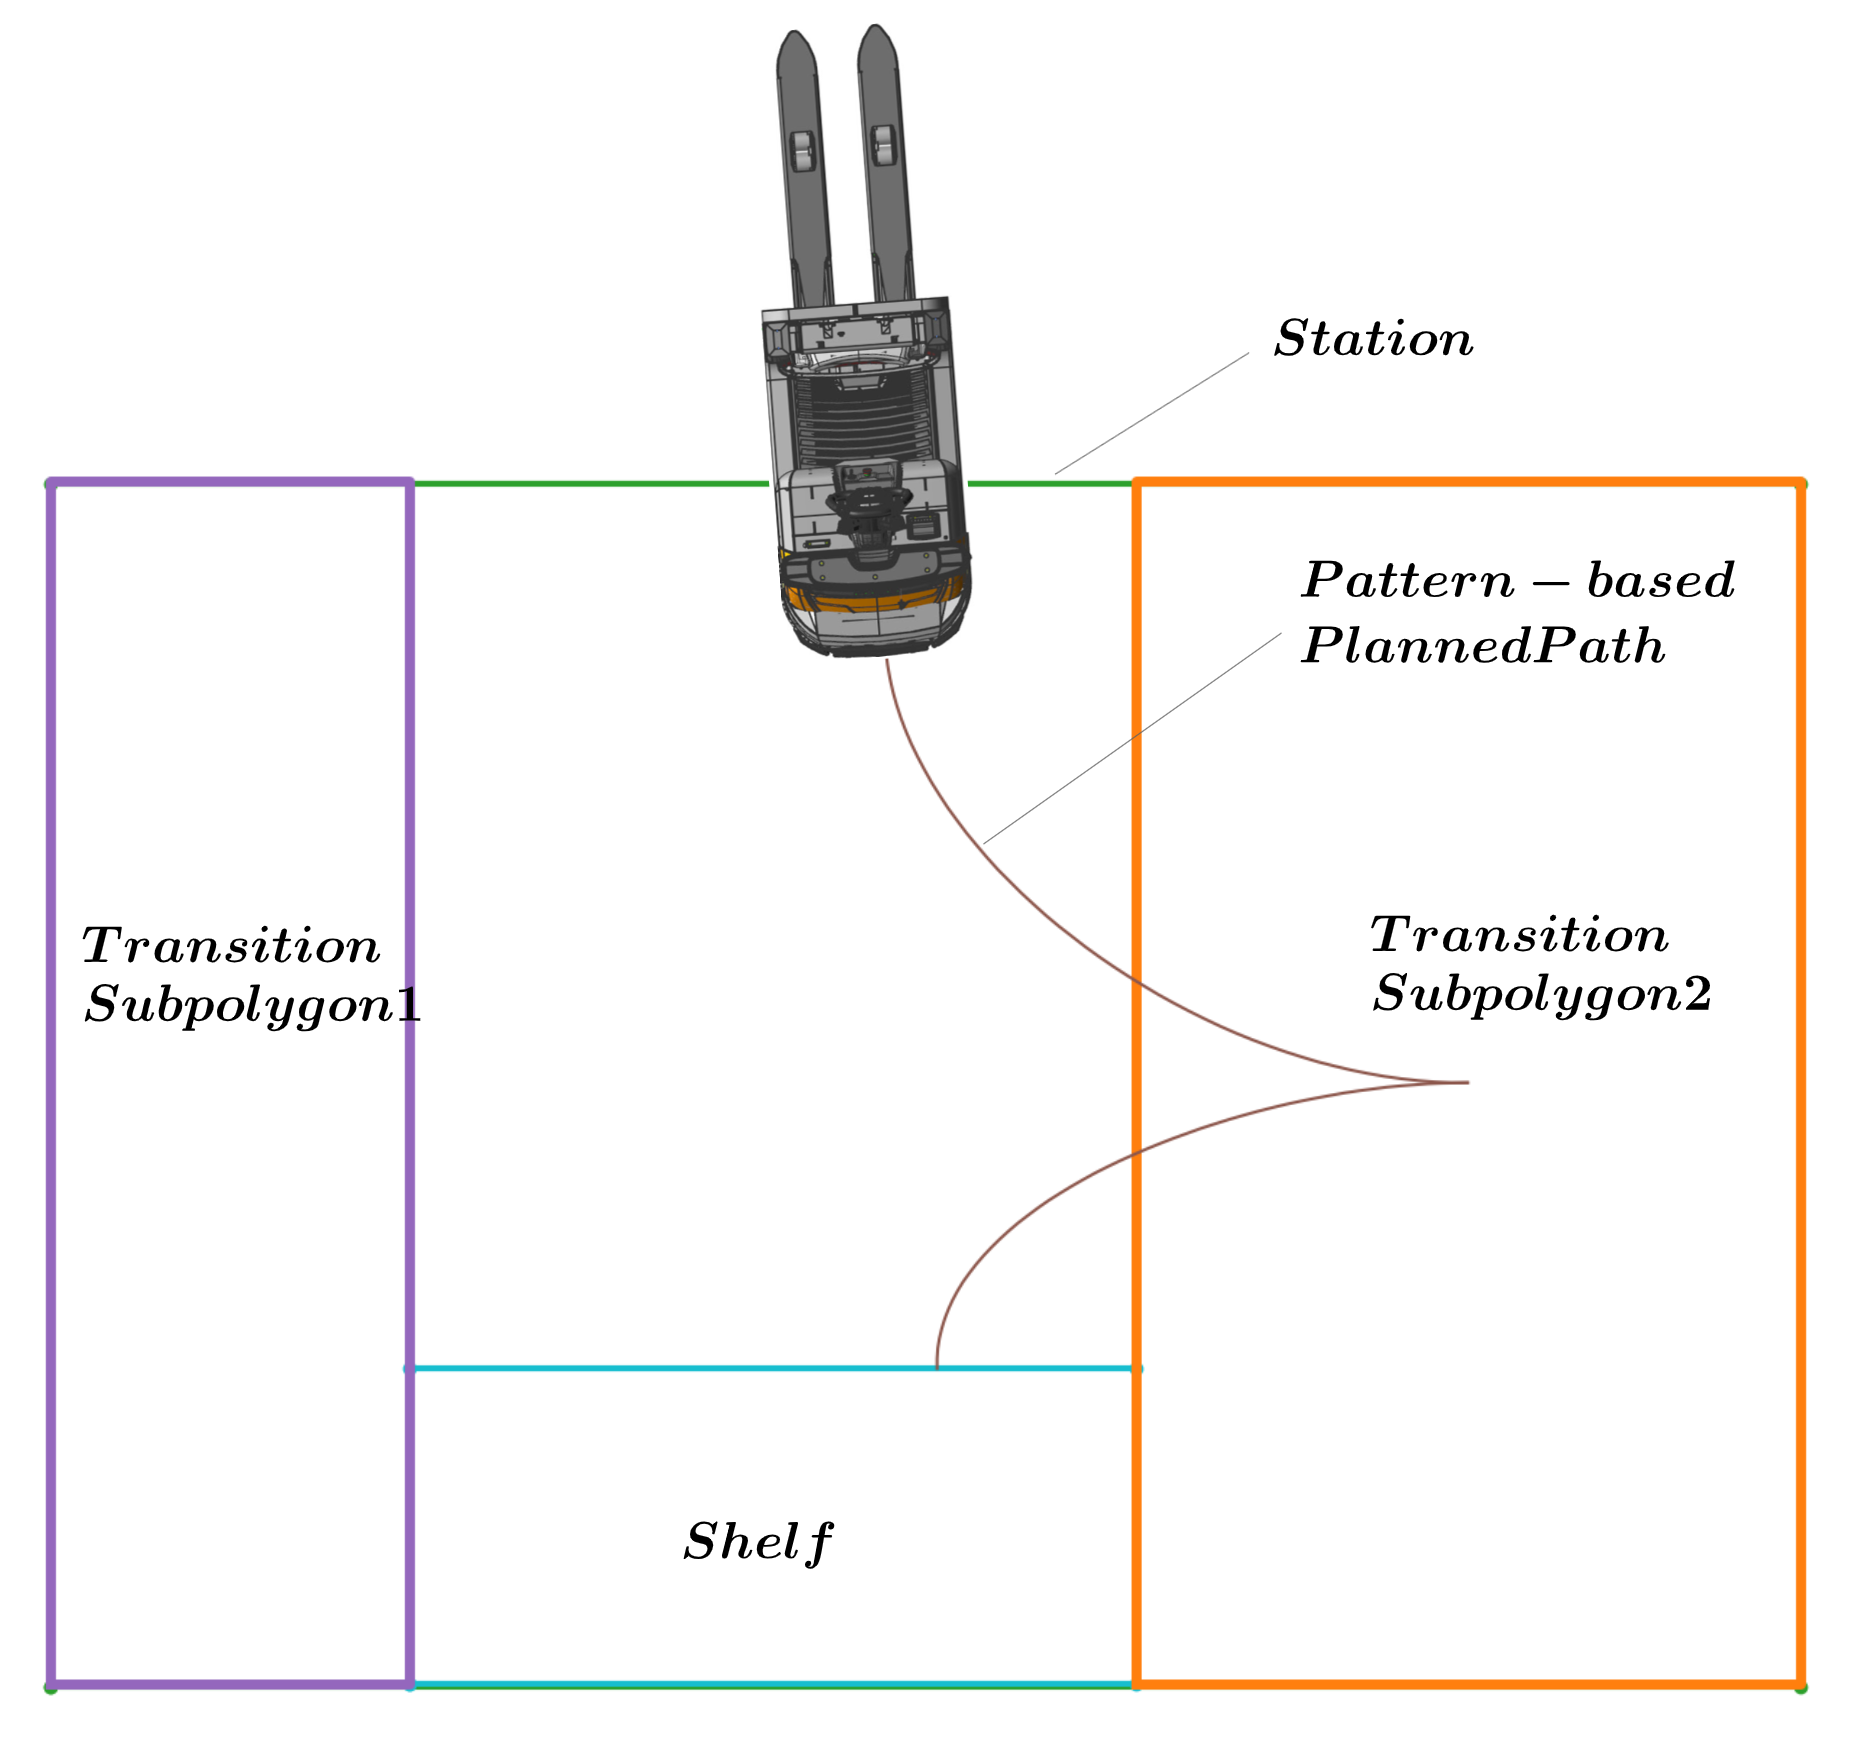
\includegraphics[width=3in]{images/Chap3/station1_pattern.png} 
    \end{minipage}
    \begin{minipage}{0.45\textwidth}
        \centering
        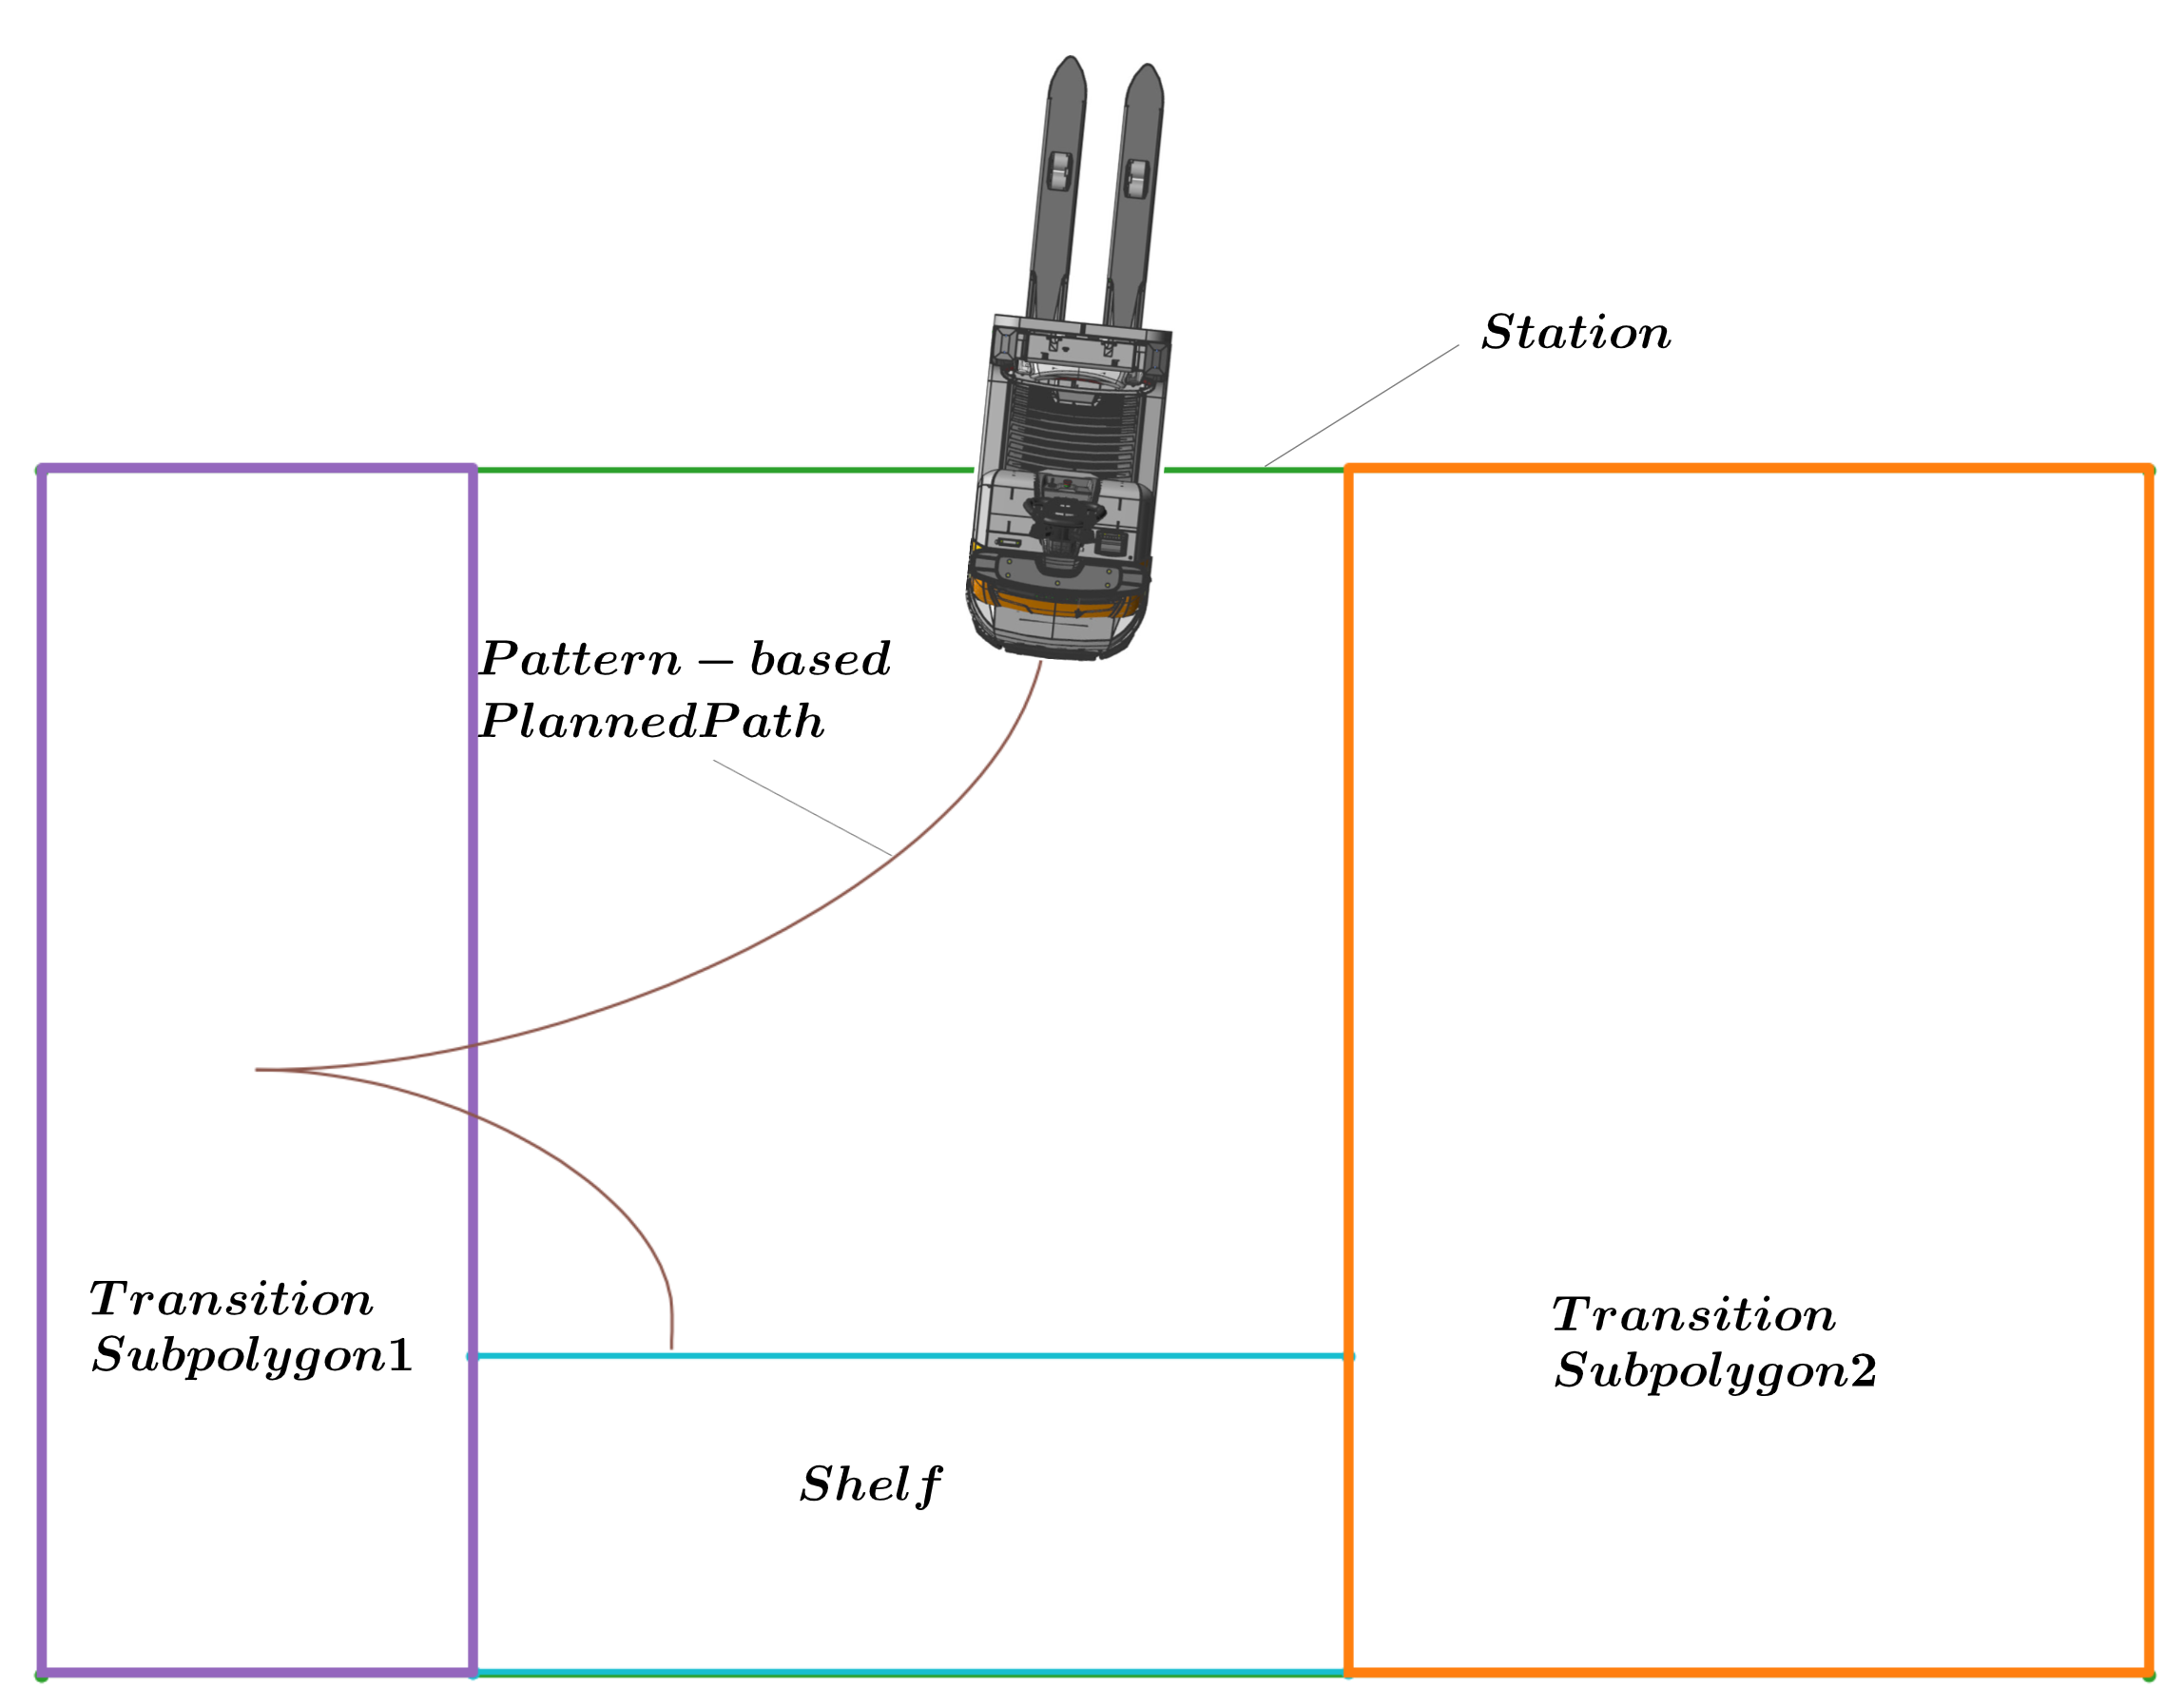
\includegraphics[width=3.5in]{images/Chap3/station2_pattern.png}
    \end{minipage}
    \caption{Test Results on Cloned Test Environment}
    \label{Test_clone}
\end{figure}

\begin{figure}[H]
    \centering
    \begin{subfigure}[b]{0.45\textwidth}
        \centering
        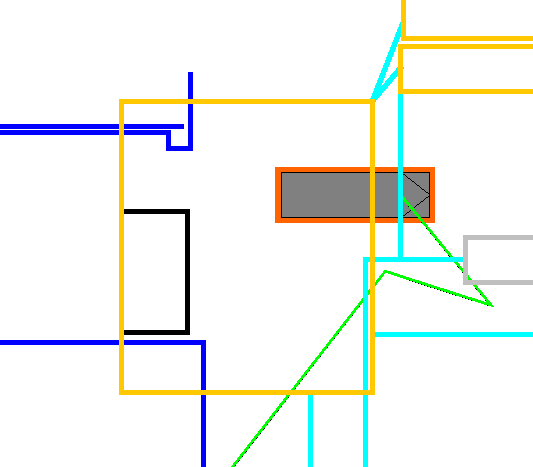
\includegraphics[width=\textwidth]{images/Chap3/Start_neksa.png}
        \caption{Test Results on the Simulated Environment: Truck at the start position}
        \label{fig:start}
    \end{subfigure}
    \hfill
    \begin{subfigure}[b]{0.45\textwidth}
        \centering
        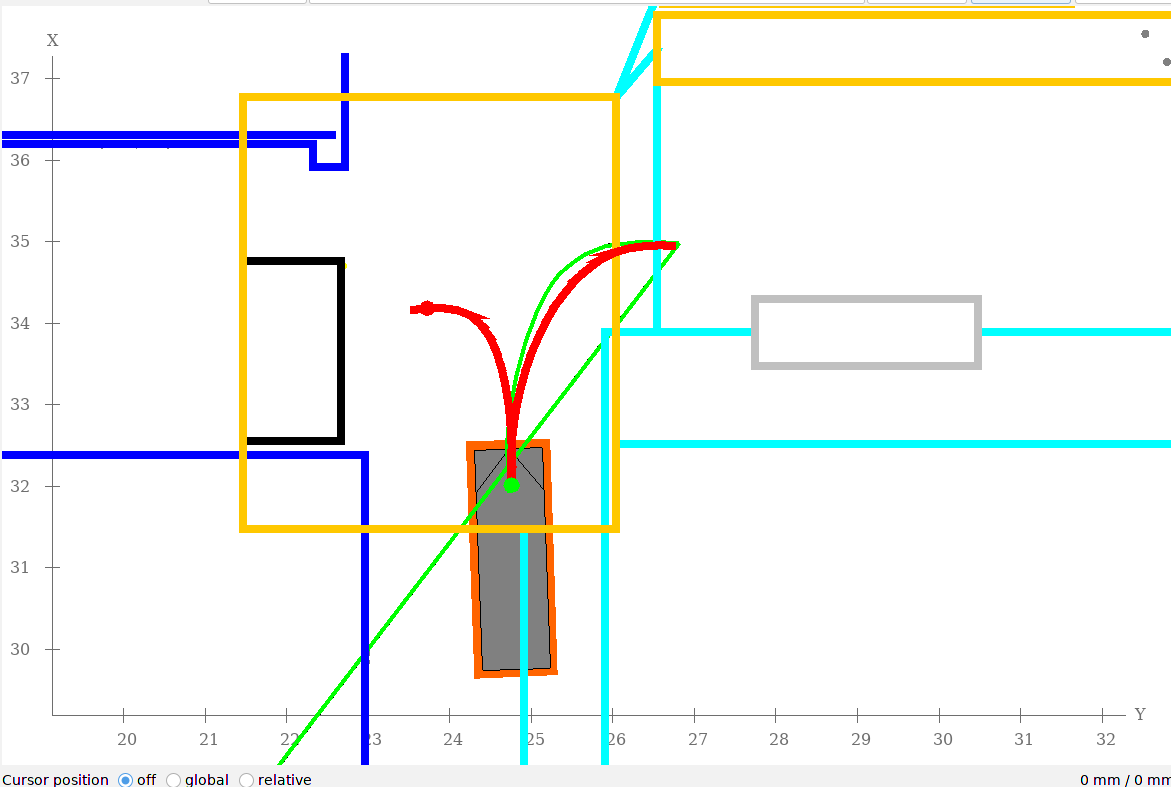
\includegraphics[width=\textwidth]{images/Chap2/Pattern_spline_simulation_3_driving.png}
        \caption{Test Results on the Simulated Environment: Truck driving the Spline-based Pattern path}
        \label{fig:spline}
    \end{subfigure}
    \caption{Test Results on the Simulated Environment}
    \label{TestResults}
\end{figure}

\begin{figure}[H]
    \centering
    \begin{minipage}{0.45\textwidth}
        \centering
        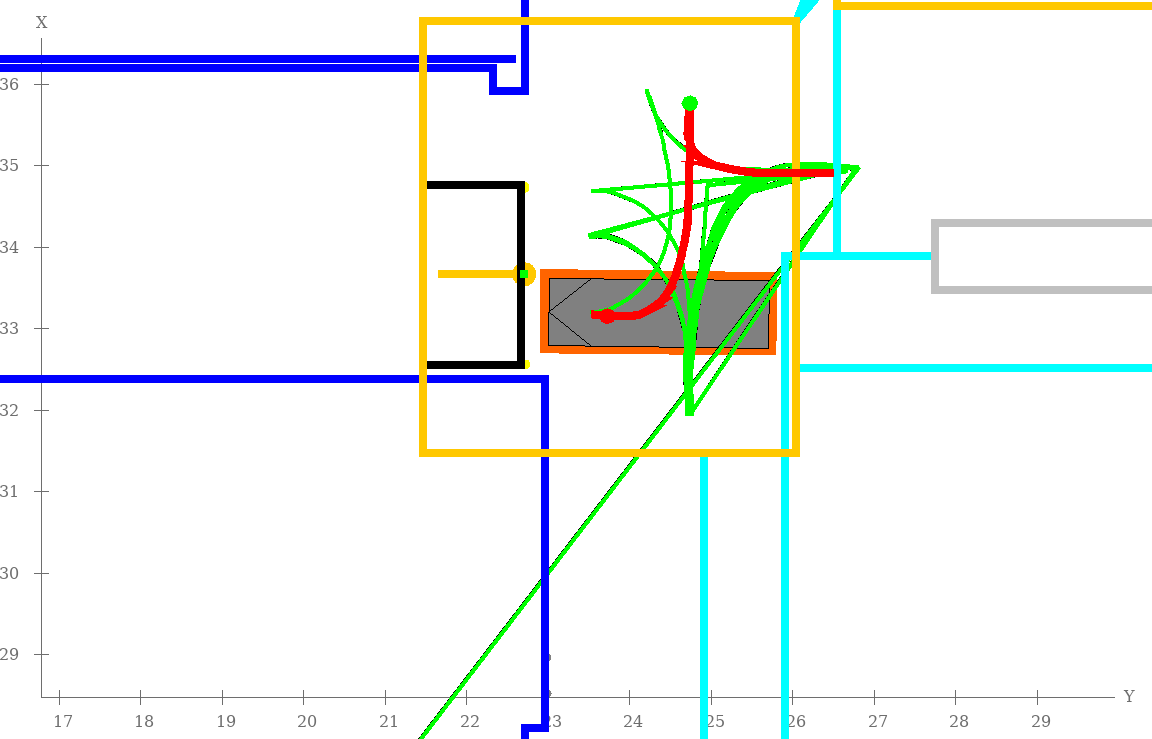
\includegraphics[width=\linewidth]{images/Chap2/Pattern_spline_simulation_1.png} % Replace with your figure
    \end{minipage}
    \begin{minipage}{0.45\textwidth}
        \centering
        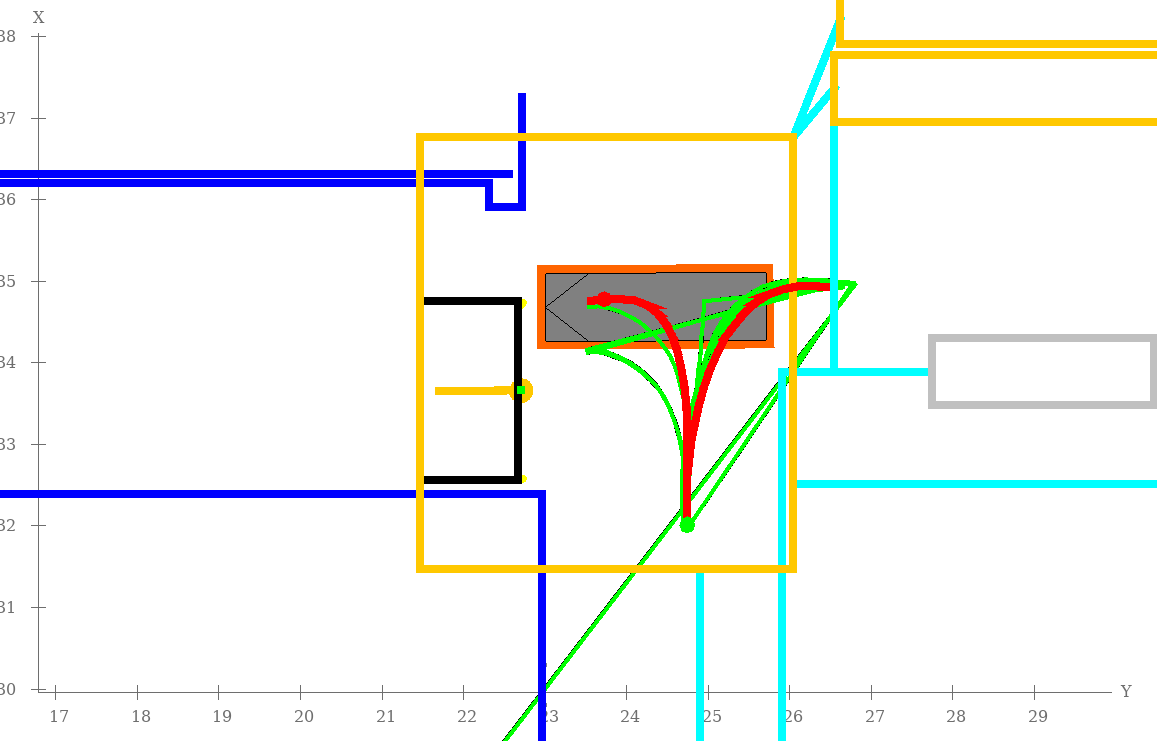
\includegraphics[width=\linewidth]{images/Chap2/Pattern_spline_simulation_2.png} % Replace with your figure
    \end{minipage}
    \caption{Test Results on the Simulated Environment: Truck at the Destination}
    \label{Test_Simu}
\end{figure}



\section{Path Evaluation Test Results and Validation}
In order to discriminate the Path Evaluation methods,
both approaches (3.3.2.1 and 3.3.2.2) were tested in the Independent Simulation Environment. 
Tests were ran on 10 different spline paths  that were generated with transition points scattered in 
the station \Ref{Mult_splines}.
Different locations of transition points were used to stress the metric outcomes by creating good and bad paths. 
The Exponential Weighted Path Evaluation was tested with \(\alpha\) = \(2\), \(\beta\) = \(0.0007\), 
\(\omega_c\)= \(0.7\) and \(\omega_L\)=\(0.3\).
The results are shown in figure \Ref{Test_Eval_Exp}: The bar chart reflects the Evaluation score of each 
spline path from figure \Ref{Mult_splines}. Each bar color reflects the same color spline.
The Normalized Weighted Path Evaluation was ran for two tests on the same splines set with:
\begin{itemize}
    \item \(\omega_c\)= \(0.7\) and \(\omega_L\)=\(0.3\)
    \item \(\omega_c\)= \(0.5\) and \(\omega_L\)=\(0.5\). 
\end{itemize}
 
The results are shown in figures \Ref{Test_Eval_Norm1} and \Ref{Test_Eval_Norm2}
%comment on results:

For the Exponential Weighted Path Evaluation, the results are correct. It is easy to differentiate poor-quality paths. 
For example, the Blue spline was used as the reference path, while the Orange, Gray, and Purple paths were intentionally 
created as bad paths. The Orange and Gray paths generate significant curvature near the destination, making it 
challenging for the vehicle to navigate and arrive in the correct position and orientation given the narrow aisle 
that it has to turn and navigate in as shown by figure  \Ref{curv_problem}. Given the high curvature and the proximity to the
destination, the truck decelerates and moves very slowly. Changes that it stops at the correct orientation 
that allows it to pickup the pallet are very low. Such path have to be avoided at all costs. The Purple path is longer 
and curved at the starting area. Furthermore, the Brown path demonstrates the best overall fitness. Although it is 
short, it introduces high curvatures at the transition and destination areas. Compared to the Blue and Red paths, 
the Brown path is shorter but less smooth. 
The Exponential Evaluation also favors the Dark Green path to the Pink one, even though the concentrated 
curvature at the end of the green path is high.
In conclusion, this evaluation method is very sensitive to path length and less 
sensitive to high concentrated curvatures. This is due to the high factor of the length term, in the range 
of thousands of millimeters, and the low factor of the curvature term which is around the magnitude of \(10^{-3}\).
It is inconvenient to change the factors \(\omega_c\) and \(\omega_L\) by increasing \(\omega_c\) and 
decreasing \(\omega_L\) as the difference becomes huge while it is mandatory to attribute 
importance to both factors. Besides, this Metric is very sensitive to the change of the \(\alpha\) and \(\beta\) factors.
These factors must be carefully tuned to fit all use cases and account for varying station sizes and configurations. 
However, finding factors that are scalable across different use cases is not straightforward.

\noindent On the other hand, The Normalized Weighted Path Evaluation, chose the Red path as the best fitness, 
outperforming the Blue pattern path. This is due to the remarkable less curvature of the Red path at the start 
and transition locations due to its proximity to the transition polygon and distance to the destination.
These factors allow for smooth driving along the path.
Comparing figures \Ref{Test_Eval_Norm1} and \Ref{Test_Eval_Norm2}, the approach of outweighing the curvature 
over the length outperforms the equal weights approach. The Pink path is visibly better than the Brown due 
to better smoothness and the first weights approach discriminates them better. 
Given the challenges associated with driving along smooth paths, it is a strategic decision to prioritize the 
curvature term over the length term. Navigating a slightly longer path is far less difficult than handling a path 
with sharp curves.
This approach is not affected by the difference of range between length and curvature metrics given that 
they are each divided respectively by the reference path's length and curvature. This not only balances out the 
two terms but also makes it fit all use cases and account for varying station sizes and configurations given that 
the reference path is always relevnat to the present station.

As a final point, \textbf{the selected approach is the Normalized Weighted Path Evaluation} with \(\omega_c\)= \(0.7\) 
and \(\omega_L\)=\(0.3\) given by equation \Ref{Norm_function}.

The Path Evaluation Approach is validated and can be used for the path Optimization phase.
The approach was validated for the following reasons: 
\begin{itemize}
    \item The Selected Evaluation method satisfies the goal of optimizing path length and thus travel time
    and limiting high curvature and challenging turns of the bulky truck by optimizing curvature change.
    \item Using the Evaluation Method, good and poor quality pattern paths can be discriminated by 
    affecting a score to each path according to its properties and comparing them.
\end{itemize}

The approach is ready to be used as the cost function of the optimizer.

\begin{figure}[H]
    \begin{center}
        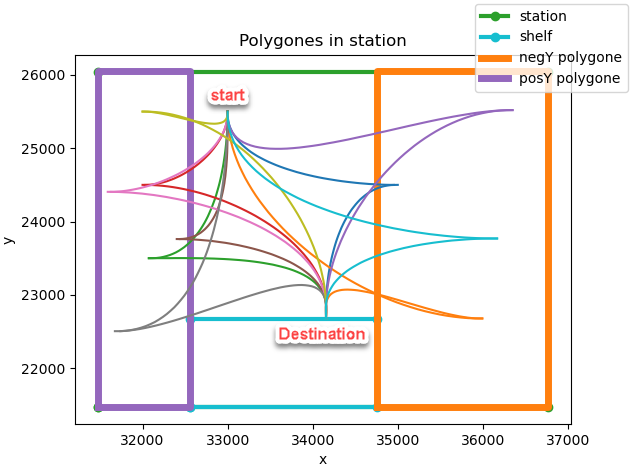
\includegraphics[width=4in]{images/Chap2/Mult_Splines_noted.png} % Replace with your figure
        \caption{Test Results on the Simulated Environment: Multiple Splines Visualization}
        \label{Mult_splines}
        \end{center}    
\end{figure}

\begin{figure}[H]
    \begin{center}
        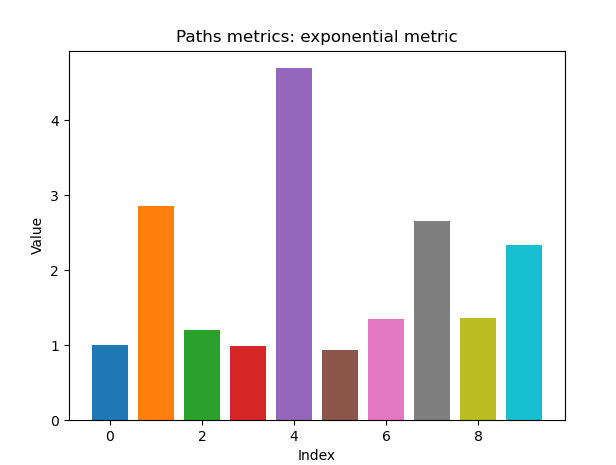
\includegraphics[width=4in]{images/Chap2/Exp_Results.png} % Replace with your figure
        \caption{Test Results on the Simulated Environment: Evaluation results of the Exponential Approach}
        \label{Test_Eval_Exp}
        \end{center}    
\end{figure}

\begin{figure}[H]
    \begin{center}
        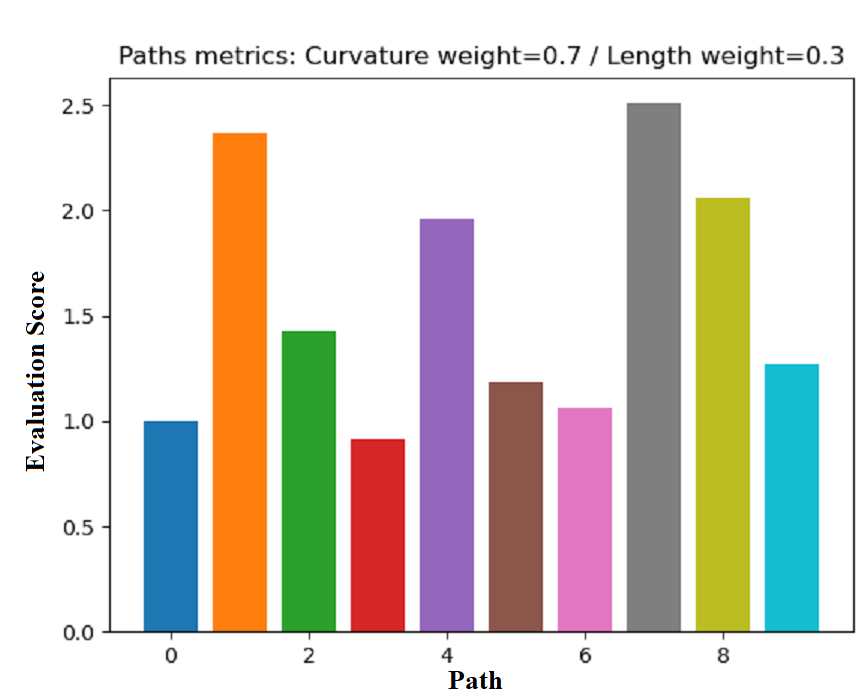
\includegraphics[width=4in]{images/Chap2/w_0.7.png} % Replace with your figure
        \caption{Test Results on the Simulated Environment: Evaluation results of the Normalized Approach
        with weighing out the curvature}
        \label{Test_Eval_Norm1}
        \end{center}    
\end{figure}
\begin{figure}[H]
    \begin{center}
        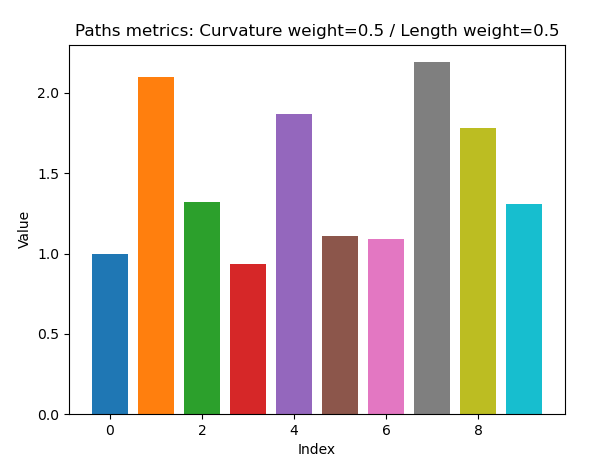
\includegraphics[width=4in]{images/Chap2/w_0.5.png} % Replace with your figure
        \caption{Test Results on the Simulated Environment: Evaluation results of the Normalized Approach
        with equal weights}
        \label{Test_Eval_Norm2}
        \end{center}    
\end{figure}

\begin{figure}[H]
    \begin{center}
        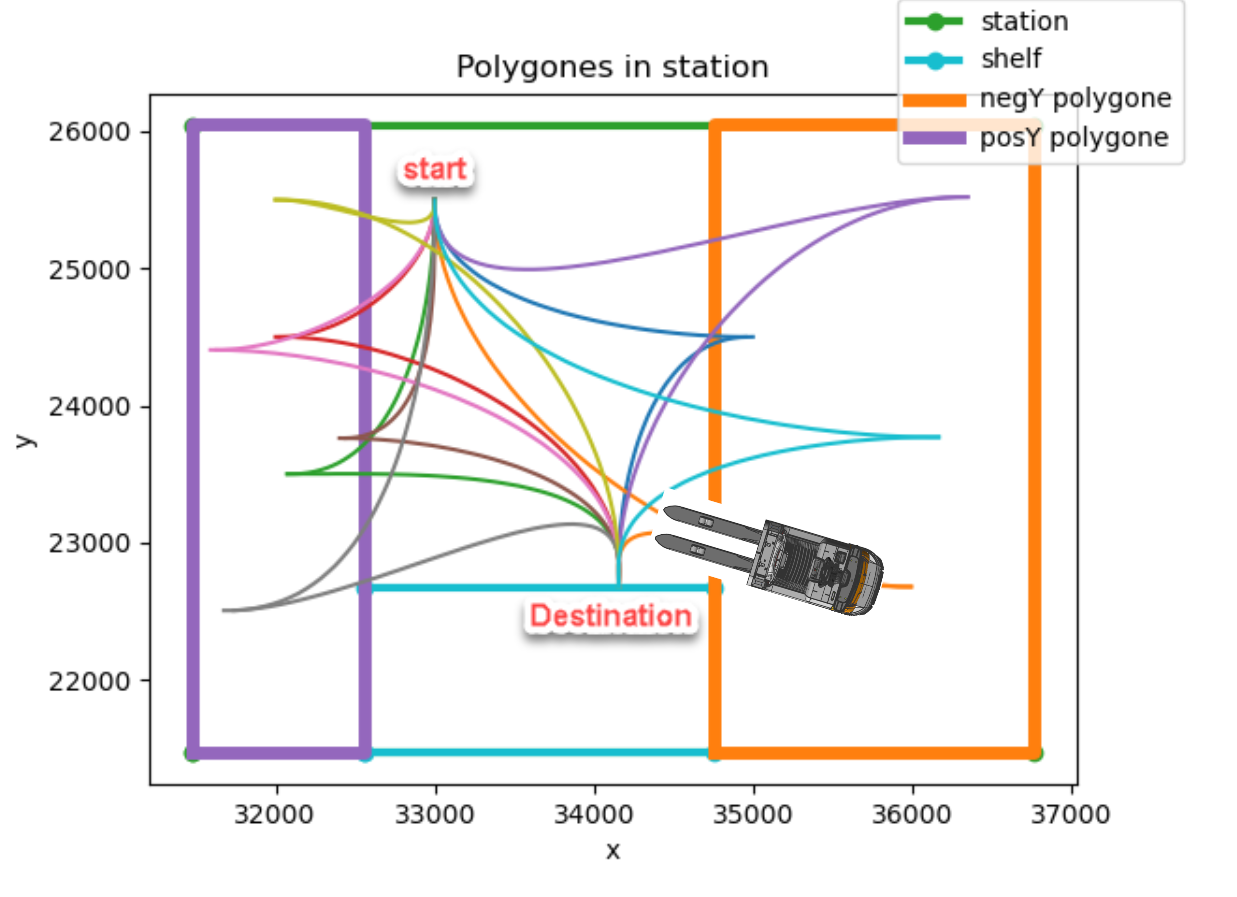
\includegraphics[width=4in]{images/Chap2/curv_problem.png} % Replace with your figure
        \caption{Navigating high curvatures in narrow areas}
        \label{curv_problem}
        \end{center}    
\end{figure}

\section{Path Optimization Test Results and Validation}

Using the Path Creation and the Selected Evaluation approach, the optimization approach is tested.
First the Optimizer is tested in an empty station, then it is tested against obstacles placed inside the station 
in different locations. 
The optimization algorithm is ran first on The 
Independent Simulation Environment to verify the relevance of the optimization approach to the pattern-based 
path. 
For this test, The Optimizer evaluates 10 generations of 10 paths for each subpolygon, it calculates the fitness value 
for each path and saves the overall best fitness value from both subpolygons. 
Figure \Ref{OptResult1} shows the result inside the Independent Simulation Environment for a station empty of obstacles:
The figure illustrates the candidate paths of the first of the 10 generations, along with the optimum paths from 
both subpolygons in bold Red and Brown "champion paths" as called in the algorithm. 
The algorithm successfully rejects poor quality paths like the lowest right red path which has two direction changes 
along the path due to the sharp turn in the beginning, and the highest left blue path that 
has an unfeasible sharp turn at the target.
The approach is validated at this stage. 

\begin{figure}[H]
    \begin{center}
        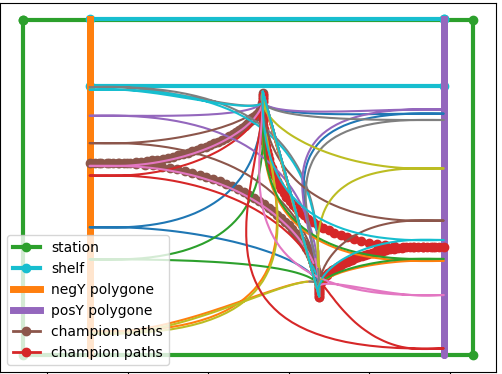
\includegraphics[width=4in]{images/Chap3/Gen1_crop.png} % Replace with your figure
        \caption{Optimizer results in empty station of one of 10 generations with the overall best paths 
        visualized in bold red and brown}
        \label{OptResult1}
        \end{center}    
\end{figure}


The second test is ran with obstacles placed in different positions in the station. 
The Algorithm results on figure \Ref{OptResult2} illustrate that the optimizer is capable of generating paths the avoid 
obstacles. The optimizer does generate paths that cross the quadrilateral obstacle but those paths 
are eliminated by better quality paths: the optimum paths in Brown. The quadrilateral obstacle was placed 
in a critical area, the center of the station to stress the optimizer. On the other hand, 
the rectangle obstacle was placed in the right corner of the station at a far distance from the start position,
the optimal transition area inside the subpolygon, and the target.
Although the two paths are  correct, the brown path is highly curved at the beginning because it avoids the 
quadrilateral obstacle. However, the red path is smoother at the start and destination segments of the path.

\begin{figure}[H]
    \begin{center}
        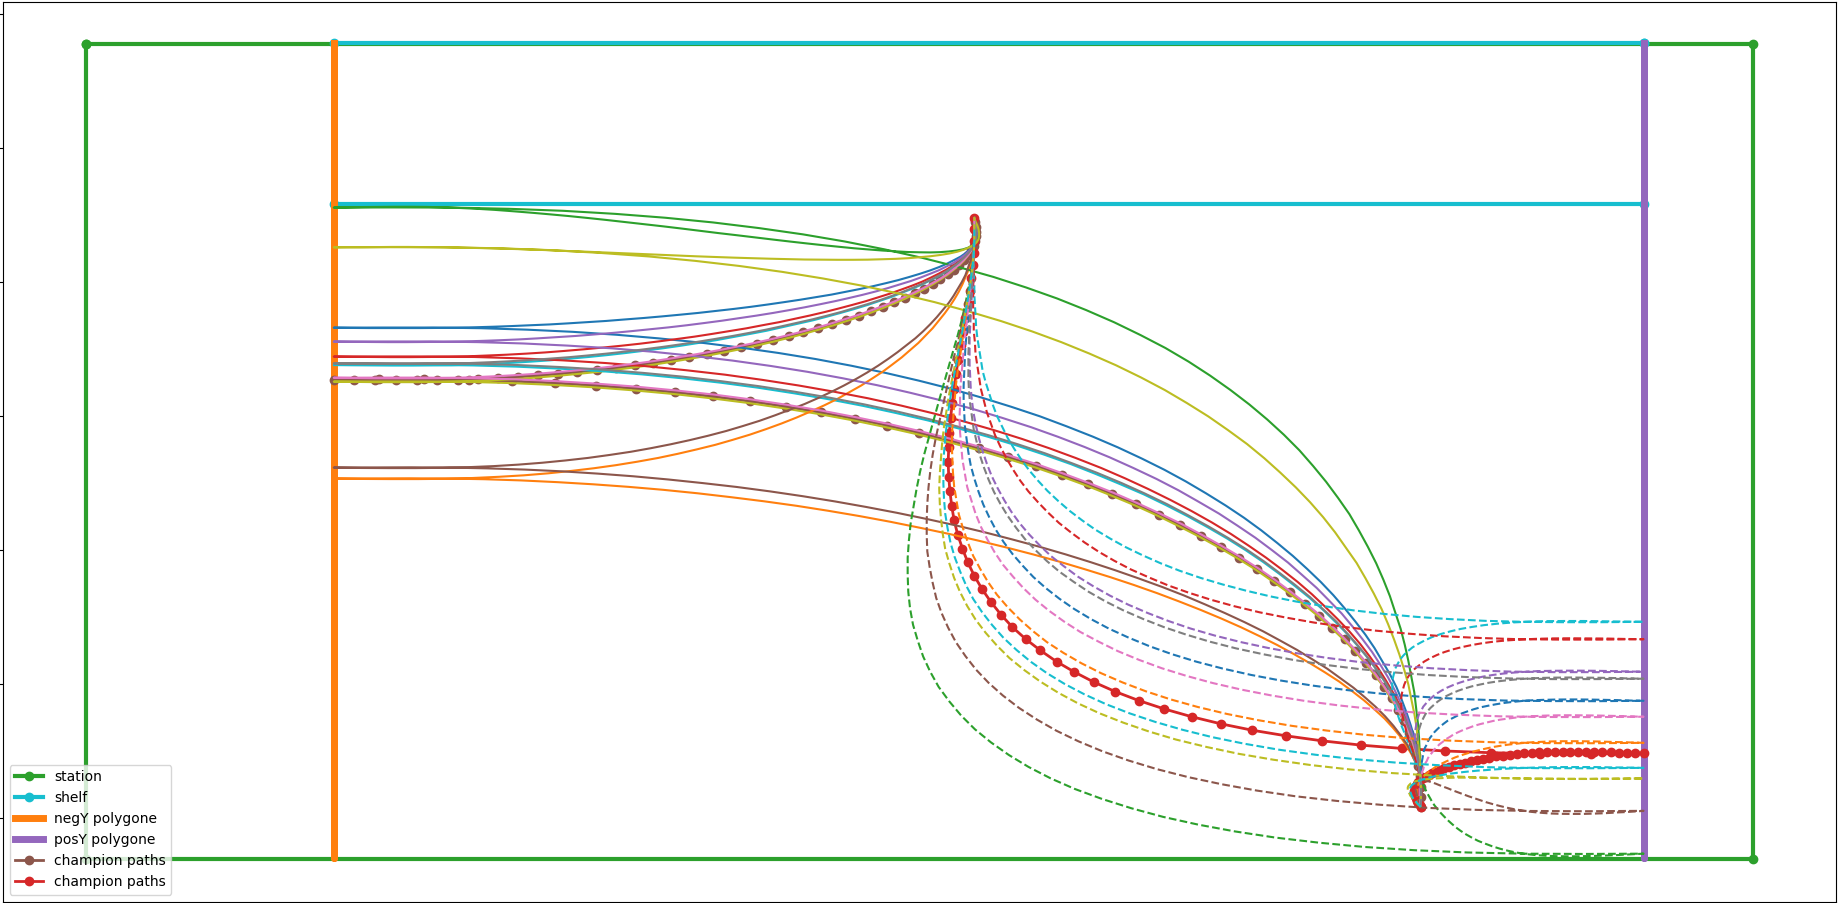
\includegraphics[width=5in]{images/Chap3/scenario3_crop.png} % Replace with your figure
        \caption{Optimizer results in presence of obstacles of one of 10 generations with the overall best paths 
        visualized in bold red and brown}
        \label{OptResult2}
        \end{center}    
\end{figure}

Another obstacle situation was tested and illustrated by figure \Ref{OptResult3}.
The obstacles in this situation were placed in the center of the station . 
For this case the regular optimizer was unable to find a solution that does not collide 
with the obstacles. However, by increasing the number of the waypoints (approach in section 3.4.2.1),
The optimizer was effective in finding collision free paths. 


\begin{figure}[H]
    \begin{center}
        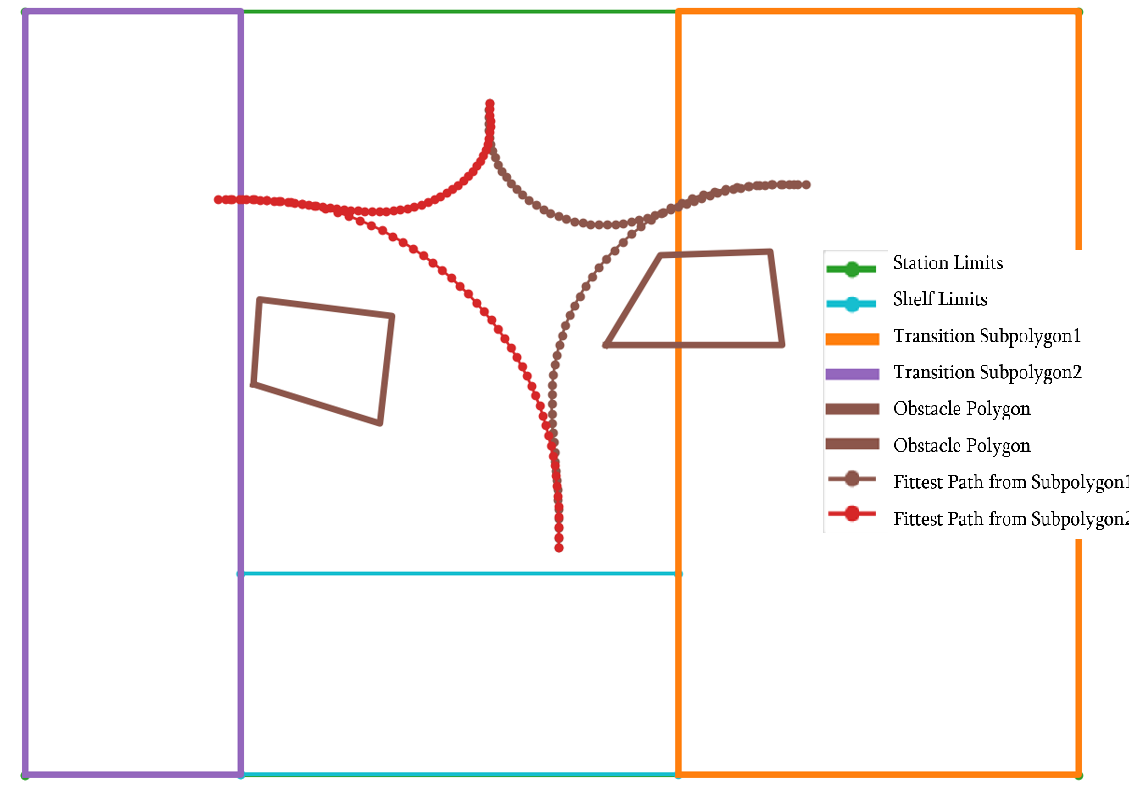
\includegraphics[width=4in]{images/Chap3/Figure_6.png} % Replace with your figure
        \caption{Optimizer results in presence of obstacles and influence of increasing path waypoints}
        \label{OptResult3}
        \end{center}    
\end{figure}

The approach is validated for a moderate complexity environment.

Given that the approach was validated in the Independent Simulation Environment, the tests are 
ran on the RACK Simulation Environment. Two test scenarios are created: 
The first is called the \(Simple~Environment\) which is an obstacle-free station and the second is
called the \(Complex~Environment\) where an obstacle is placed in one side of the station. 
In reality, the \(Simple~Environment\) is not simple because the sensors detect the warehouse walls,
shelves, objects, and other vehicles, but the station area is free of stranger objects.
The test in the \(Simple~Environment\) illustrated by figure \Ref{OptResult4} was done by placing the 
AMR in the simulation in the starting position (green rectangle) and selecting the target position on 
the simulation model. The expected target position is the red rectangle. 
The path is planned following the pattern and links the AMR from its start position to the target position.
The blueprints along the path represent the positions that the AMR will be at when driving the path.
The footprint helps to ensure that the AMR will not collide with surrounding objects and 
validate the optimizer's ability to avoid obstacles. 

\begin{figure}[H]
    \begin{center}
        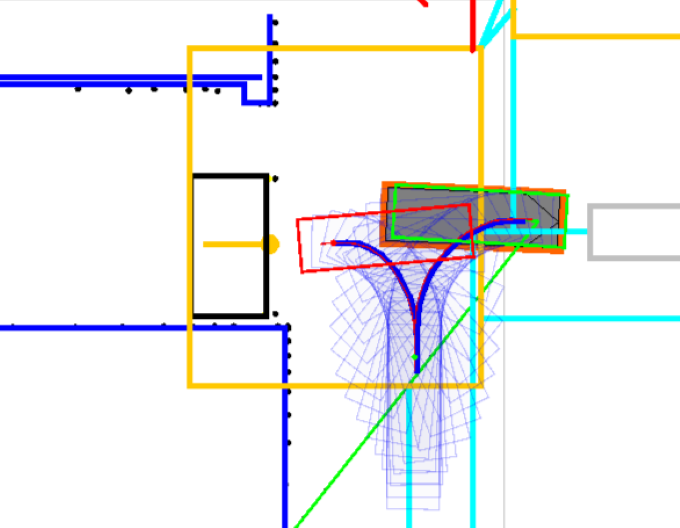
\includegraphics[width=4in]{images/Chap3/Start.png} % Replace with your figure
        \caption{Optimizer results in a simple environment tested inside the RACK simulation: Start Position}
        \label{OptResult4}
        \end{center}    
\end{figure}

\begin{figure}[H]
    \begin{center}
        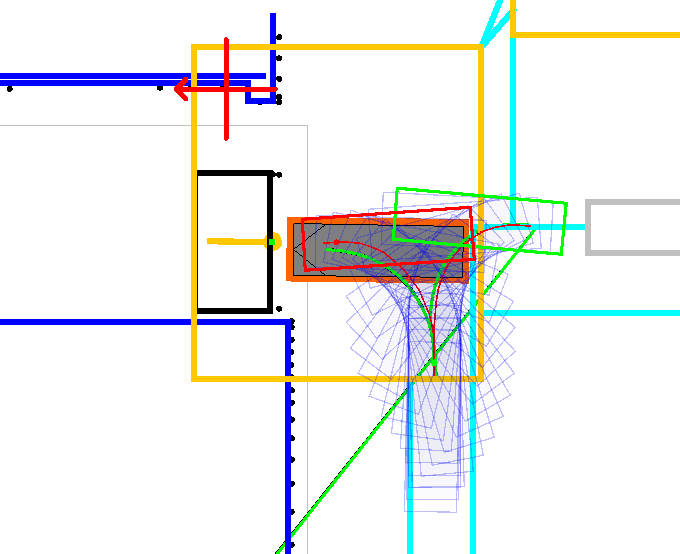
\includegraphics[width=4in]{images/Chap3/Target.png} % Replace with your figure
        \caption{Optimizer results in a simple environment tested inside the RACK simulation: Target Position}
        \label{OptResult5}
        \end{center}    
\end{figure}

As for the \(Complex~Environment\), an obstacle was placed at the side of the station 
blocking one of the subpolygons as illustrated in figure \Ref{OptResult6}: the blue rectangle at the bottom 
of the figure.
The planned pattern path (red path) transitions in the opposite subpolygon as it is clear of obstacles.
The optimizer successfully generates a pattern path that avoids known obstacles such as the shelf and 
the warehouse walls as well as new obstacles like the blue rectangle. 
The generated path is aligned with the kinematic constraints of the vehicle as illustrated on figure \Ref{OptResult7}: 
it avoids highly curved turns and limits the direction changes to one thus ensuring a smooth navigation.
Finally, the truck docks the target location at the desired position as shown in figure \Ref{OptResult8}: 
The forks are facing the shelf and ready to start pick up/ drop process. 

\textbf{Remark}: the shift of the final position of the vehicle on figure \Ref{OptResult8} is due 
to control issues. Currently, the path following is not completely correct and requires 
control improvement.

\begin{figure}[H]
    \begin{center}
        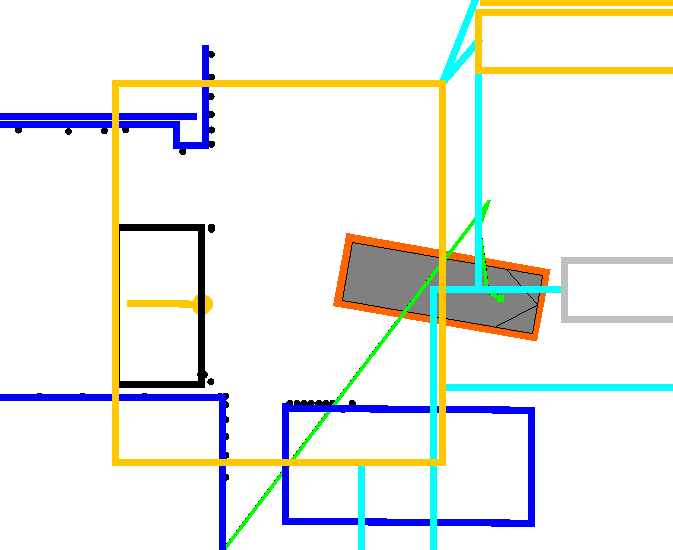
\includegraphics[width=4in]{images/Chap3/4.png} % Replace with your figure
        \caption{Optimizer results in a Complex environment tested inside the RACK simulation: Start Position}
        \label{OptResult6}
        \end{center}    
\end{figure}

\begin{figure}[H]
    \begin{center}
        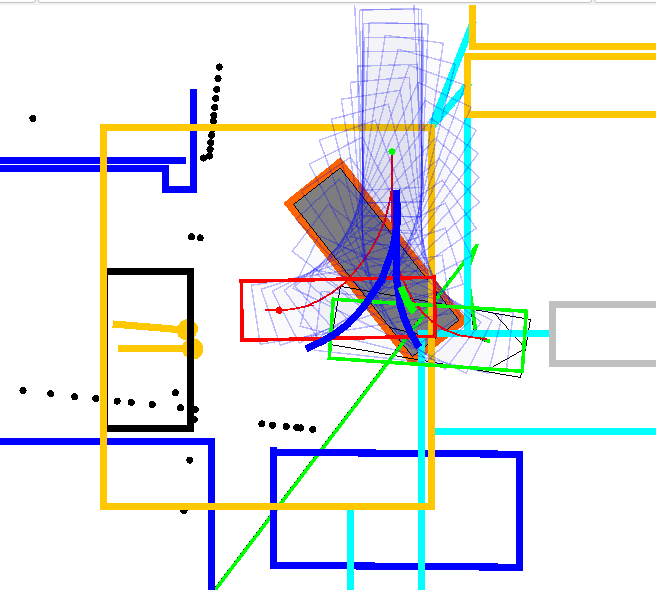
\includegraphics[width=4in]{images/Chap3/2.png} % Replace with your figure
        \caption{Optimizer results in a Complex environment tested inside the RACK simulation: AMR Navigating the path}
        \label{OptResult7}
        \end{center}    
\end{figure}

\begin{figure}[H]
    \begin{center}
        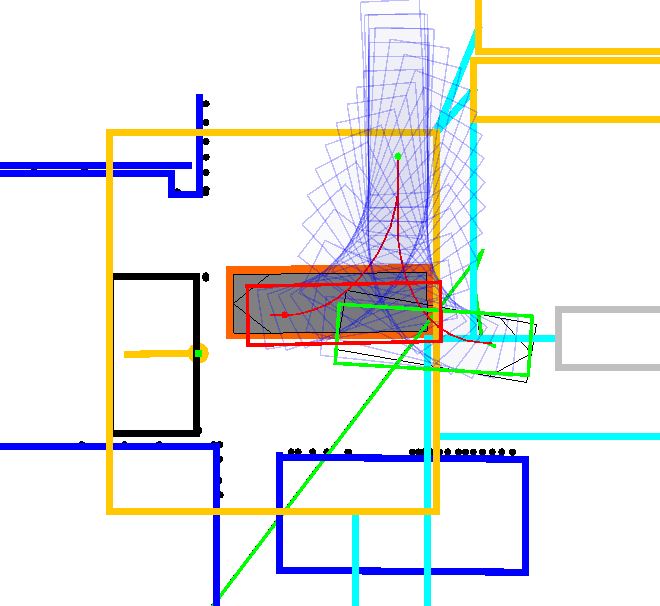
\includegraphics[width=4in]{images/Chap3/3.png} % Replace with your figure
        \caption{Optimizer results in a Complex environment tested inside the RACK simulation: Target Position}
        \label{OptResult8}
        \end{center}    
\end{figure}

Using the \(Simple~Environment\) and the \(Complex~Environment\) tests were ran inside the 
RACK Simulation Environment to compare the performance of the Metaheuristic Algorithms: GA, DE, PSO,
ACO, and SA. 

The same starting and Target Positions were used for each scenario. For the \(Complex~\\Environment\),
the same obstacle was used for all the algorithm tests to create the same test conditions, the obstacle used is 
marked in green on figure \Ref{OptResult9}. All algorithms were configured to evolve around 200 candidates.
The comparison between the Algorithms in the simulation is based on: 
\begin{itemize}
    \item The Planning Time: the time that each algorithm takes to evolve a solution.
    \item The Created Path's Fitness Values.
\end{itemize}

Table \Ref{tab:planning_time} shows the planning times for simple and complex Environment 
for each algorithm. 
For the Simple Environment, the DE algorithm prevails at a planning time of \(27ms\).
The worst planning time is with the SA algorithm at \(80ms\). 
GA, PSO, and ACO have the same range of Planning time \(56\) to \(59ms\).
For the complex Environment, The raking is the same: the best algorithm in terms of planning time 
is the DE at \(44ms\), next comes the ACO at \(65ms\). The least performing algorithm remains the SA 
with a planning time of \(78ms\). It is noticeable that the planning time increased overall
for almost all the algorithms in the complex environment scenario. 
This is due to the checking of the scan points that increase as more objects are introduced around the AMR.

Using the planning time based comparison the DE algorithm is the most performing in terms of planning time. 

Table \Ref{tab:fitness_values} details the fitness values for both scenarios. It is worth mentioning
that the obstacle is placed inside subpolygon1 in this case.
For the Simple Environment, the GA was able to find the fittest candidate at an evaluation score of 
\(0.32\) in subpolygon2, however, the DE has the highest fitness values \(0.652\) in subpolygon1 and \(0.56\) in subpolygon2 
even though it was the fastest in terms of planning time.
For the complex Environment, the PSO was the fittest with an evaluation score of \(0.38\) in subpolygon2 and very 
close was the DE with \(0.384\). As for subpolygon1 where the obstacle stands, the fitness values are very high.
The values can be clustered into two groups:
\begin{itemize}
    \item Knockout value: this is the cluster of the fitness values equal to \(50\). It was obtained
    with the ACO and DE. The knockout value is the fitness value assigned to the paths that collide with obstacles.
    Returning a fitness function of \(50\) means that the optimizer was not able to find a path at that subpolygon.
    \item High values < \(50\): For GA, PSO, and SA the fitness values are respectively \(31\), \(1.159\), and \(1.258\).
    These values are caused by penalizing the high curvatures.
    If a path's maximum curvature exceeds the maximum tolerated curvature of the truck, the Path gets penalized by 
    emphasizing it curvature. Despite the poor quality of the paths, these algorithms still found feasible solutions 
    to get around the obstacle. 
\end{itemize}

Using this comparison, the PSO algorithm outperforms the other algorithms in complex environments as it 
finds the fittest path which refers to the shortest path and the least curvature change and also finds a path in 
the constrained subpolygon where the obstacle stands.

\begin{figure}[H]
    \begin{center}
        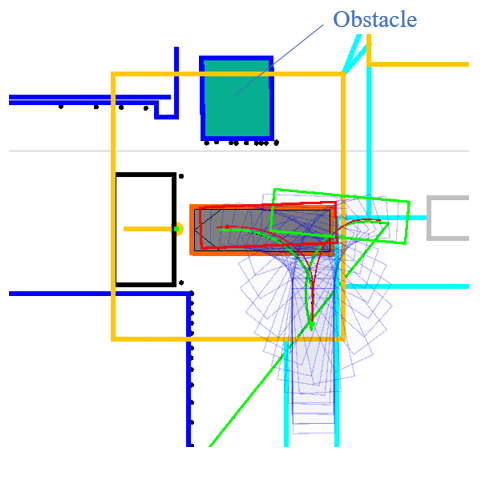
\includegraphics[width=4in]{images/Chap3/obstacle_complicated.png} % Replace with your figure
        \caption{Obstacle Used for Metaheuristic Algorithms comparison in the complex scenario}
        \label{OptResult9}
        \end{center}    
\end{figure}

\begin{table}[H]
    \centering
    \caption{Comparison of Planning Time for Different Algorithms in Simple and Complex Environments (in milliseconds)}

    \resizebox{\textwidth}{!}{%
    \begin{tabular}{|p{3.5cm}|p{5cm}|p{5cm}|}
    \hline
    \textbf{Algorithm} & \textbf{Planning Time (Simple Environment) (ms)} & \textbf{Planning Time (Complex Environment) (ms)} \\
    \hline
    Genetic Algorithm & 57 & 73 \\
    \hline
    Particle Swarm Optimization & 59 & 67 \\
    \hline
    Ant Colony Optimization & 56 & 65 \\
    \hline
    Simulated Annealing & 80 & 78 \\
    \hline
    \rowcolor{green!30} Differential Evolution & 27 & 44 \\
    \hline
    \end{tabular}%
    }
    \label{tab:planning_time}
\end{table}

\begin{table}[H]
    \centering
    \caption{Comparison of Fitness Values of the optimum paths generated by Different Algorithms in Simple and Complex Environments}

    \resizebox{\textwidth}{!}{%
    \begin{tabular}{|p{4cm}|p{2.5cm}|p{2.5cm}|p{2.5cm}|p{2.5cm}|}
    \hline
    \multirow{2}{*}{\textbf{Algorithm}} & \multicolumn{2}{c|}{\textbf{Simple Environment}} & \multicolumn{2}{c|}{\textbf{Complex Environment}} \\
    \cline{2-5}
     & \textbf{Subpolygon1 Fitness} & \textbf{Subpolygon2 Fitness} & \textbf{Subpolygon1 Fitness} & \textbf{Subpolygon2 Fitness} \\
    \hline
    Genetic Algorithm       & \cellcolor{green!30} 0.549  & \cellcolor{green!30} 0.32  & 31.0  & 0.449 \\
    \hline
    Particle Swarm Optimization  & 0.561  & 0.349  & \cellcolor{green!30} 1.159  & \cellcolor{green!30} 0.38 \\
    \hline
    Ant Colony Optimization      & 0.542  & 0.384  & 50.0  & 0.417 \\
    \hline
    Simulated Annealing     & 0.45  & 0.394  & 1.258  & 0.428 \\
    \hline
    Differential Evolution  & 0.652  & 0.56  & 50.0  & 0,384 \\
    \hline
    \end{tabular}%
    }
    \label{tab:fitness_values}    
\end{table}

\section{Field-Testing of the Solution on the AMR}
This section sums up the developed module for a field test on the iGo Neo Truck. 
First the test Conditions are outlined, then the planning process with the sensor input are explained.
Finally, the planned path and navigation of the truck in each scenario are discussed.

The Approach is tested in 3 different scenarios:
\begin{itemize}
    \item A Simple Test Environment where The station is free of obstacles.
    \item Moderate complexity Test Environments where  obstacles are placed in 2 areas of the station:
    left and right sides of the shelf. The obstacles are intended to block one subpolygon.
\end{itemize}

\subsection{Simple Test Environment}
The truck was placed at position \(x = 33026\), \(y = 28070\), and \(\rho = 100.0^\circ\) 
as illustrated by 
figure \Ref{OptResult10}.
The sensor input of the truck as scan points which detects the obstacles is represented by black points
on the figure. Figure \Ref{OptResult11} shows the start position of the Truck inside the warehouse.
The RACK simulation is now a real-time visualization of the real warehouse.
The goal is to dock the shelf which is represented in the real warehouse image \Ref{OptResult11}
by the yellow floor anchors at position \(x = 33426\), \(y = 22696\), and \(\rho = 0.0^\circ\). 
They hold the reflectors that return the shelf's position.
After station, shelf and target recognition, and station partitioning,
the optimizer starts generating and evaluating the candidate paths.
After successful processing of an optimum path, the truck start driving it.
The optimum path is illustrated on figure \Ref{OptResult50} in red. The path is followed by the truck 
that moves in opposite direction and negative speed until the transition location.
Starting from the transition location, it drives in main direction orienting the forks 
towards the shelf in preparation to dock then pickup or drop. 


\begin{figure}[H]
    \begin{center}
        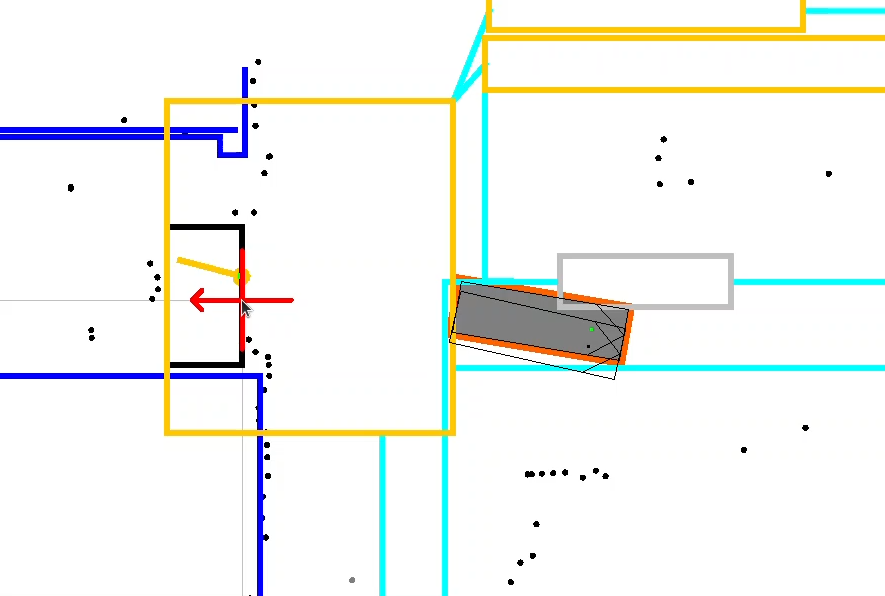
\includegraphics[width=4in]{images/Chap3/StartSimpleEnv.png} % Replace with your figure
        \caption{Environment and Start position of the Simple Test Scenario}
        \label{OptResult10}
        \end{center}    
\end{figure}


\begin{figure}[H]
    \begin{center}
        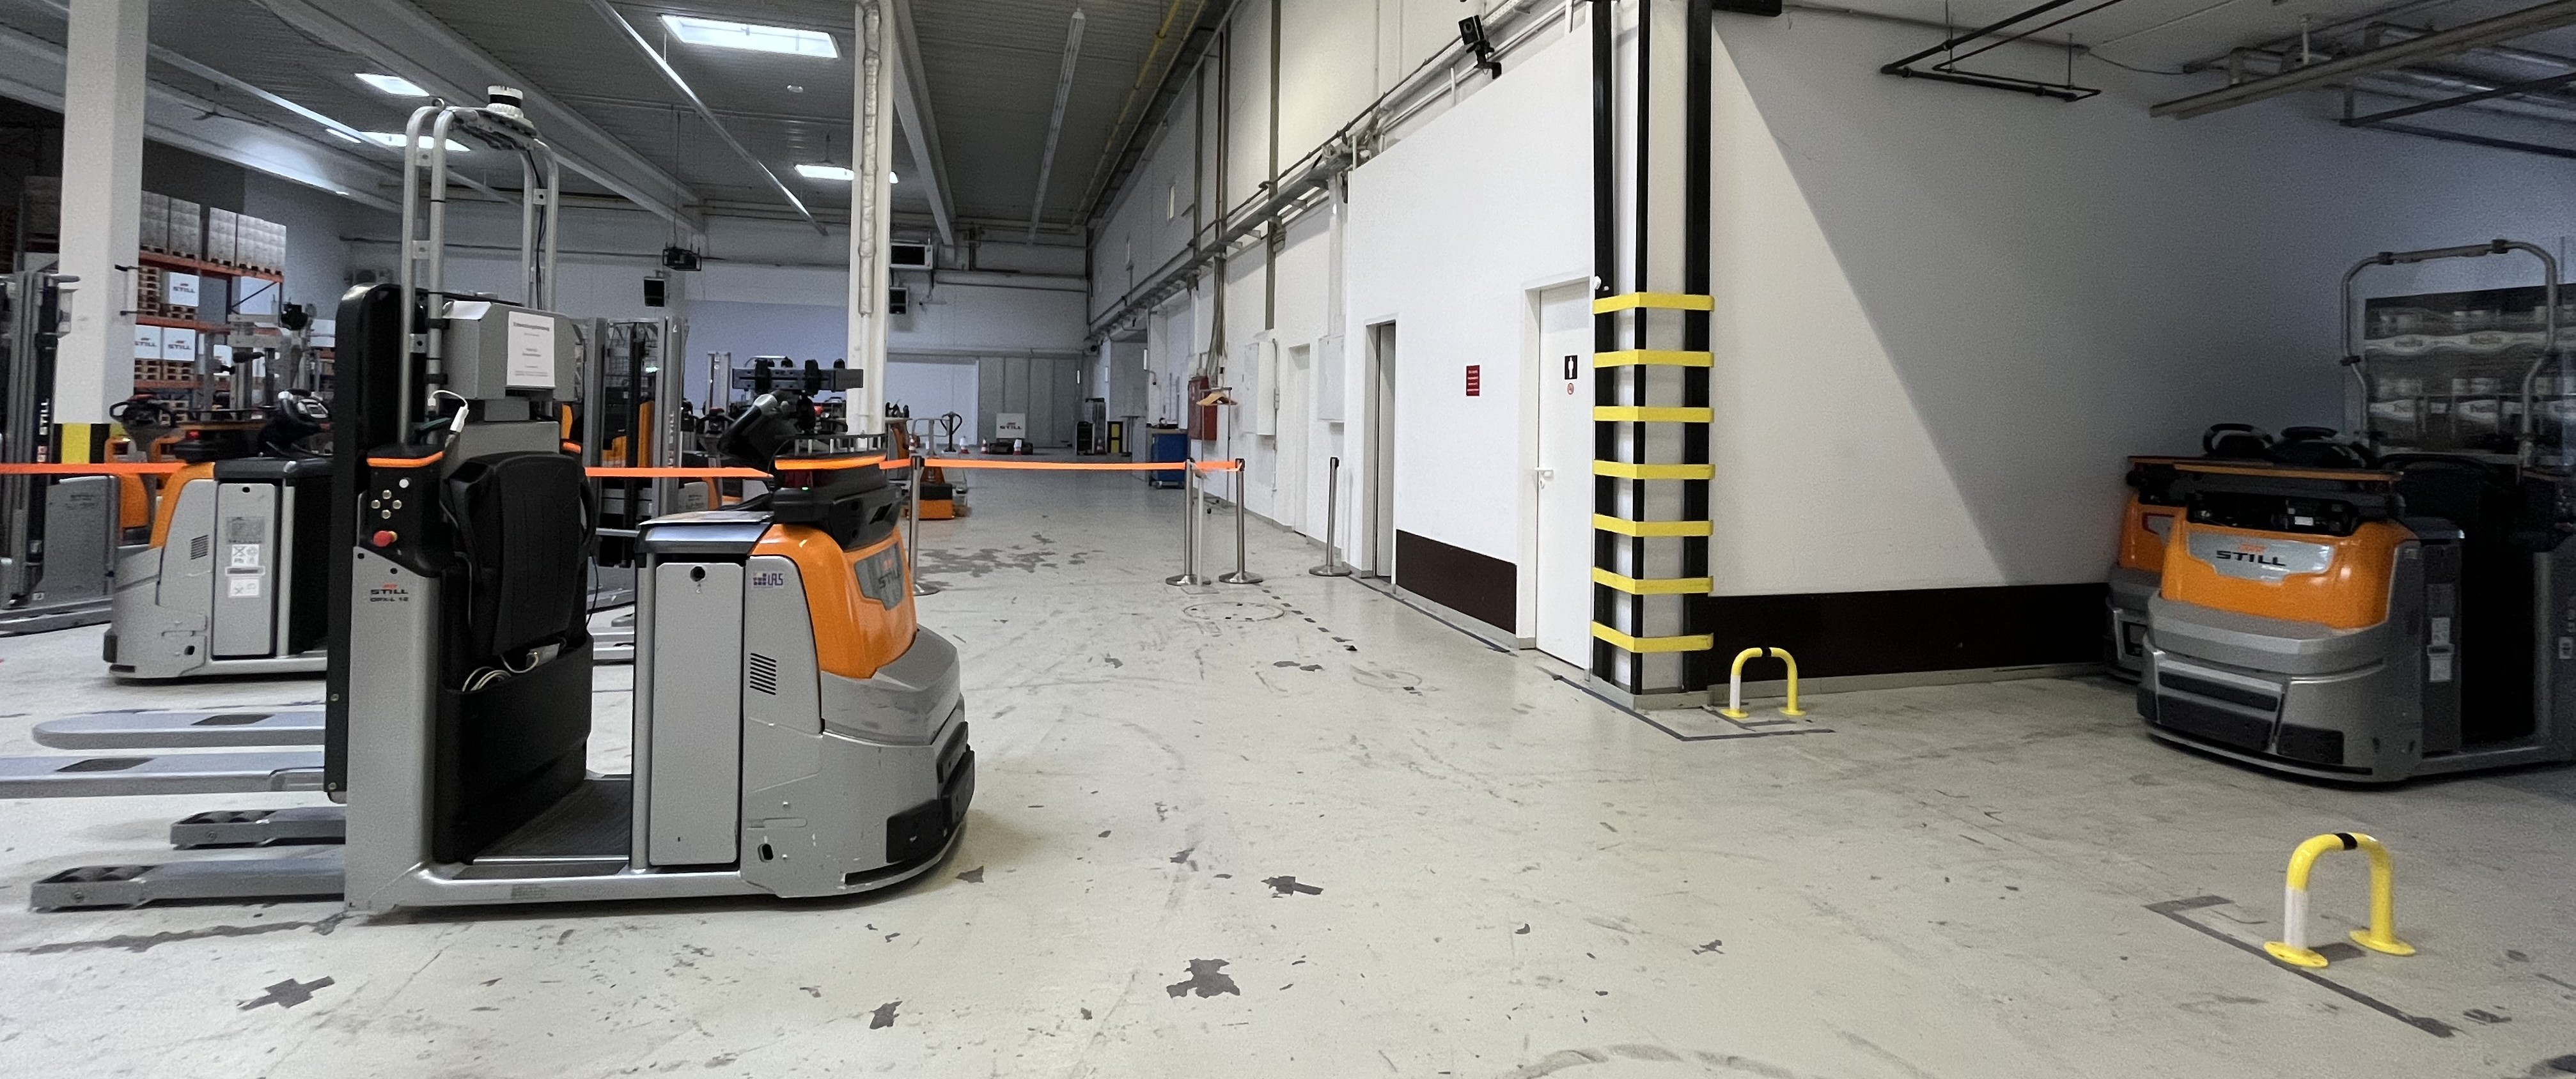
\includegraphics[width=5in]{images/Chap3/Start_Sc1.jpg} % Replace with your figure
        \caption{Environment and Start position of the Simple Test Scenario in a real warehouse
        with iGo Neo}
        \label{OptResult11}
        \end{center}    
\end{figure}

On this picture is a real warehouse where the field test took place.
The test truck is an iGo Neo and the station used is station \(Empty pallets\) at a 
global position inside the warehouse \(x = 34121\), \(y = 23752\), and \(\rho = 0.0^\circ\).
The station limits are fictional they are not outlined in the warehouse, 
but they can be seen on figure \ref{OptResult10}.
The shelf is marked by the yellow floor anchors fixed on the floor.
The environment for this test is not completely simple and empty as 
other trucks, objects, and people are in the warehouse, yet, the station is 
empty. 

\begin{figure}[H]
    \begin{center}
        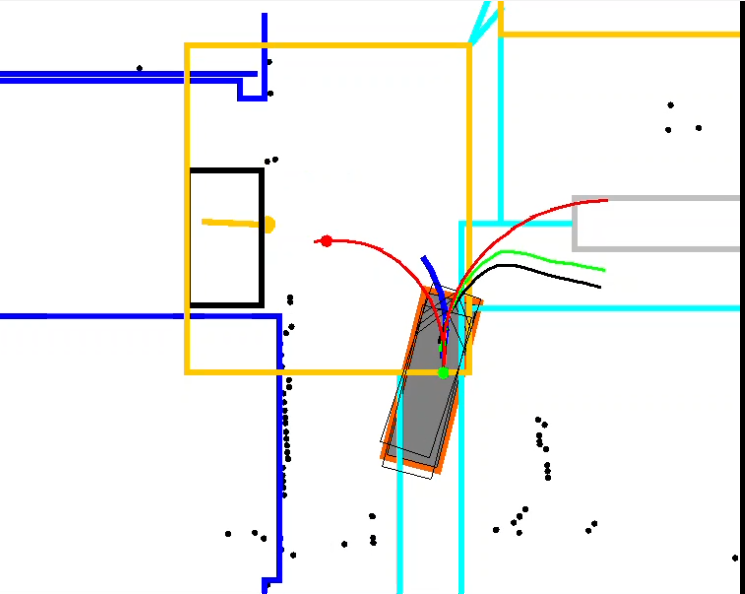
\includegraphics[width=3in]{images/Chap3/Test1_transition.png} % Replace with your figure
        \caption{Truck in the simulation navigating the planned path: Transition phase}
        \label{OptResult50}
        \end{center}    
\end{figure}


\begin{figure}[H]
    \begin{center}
        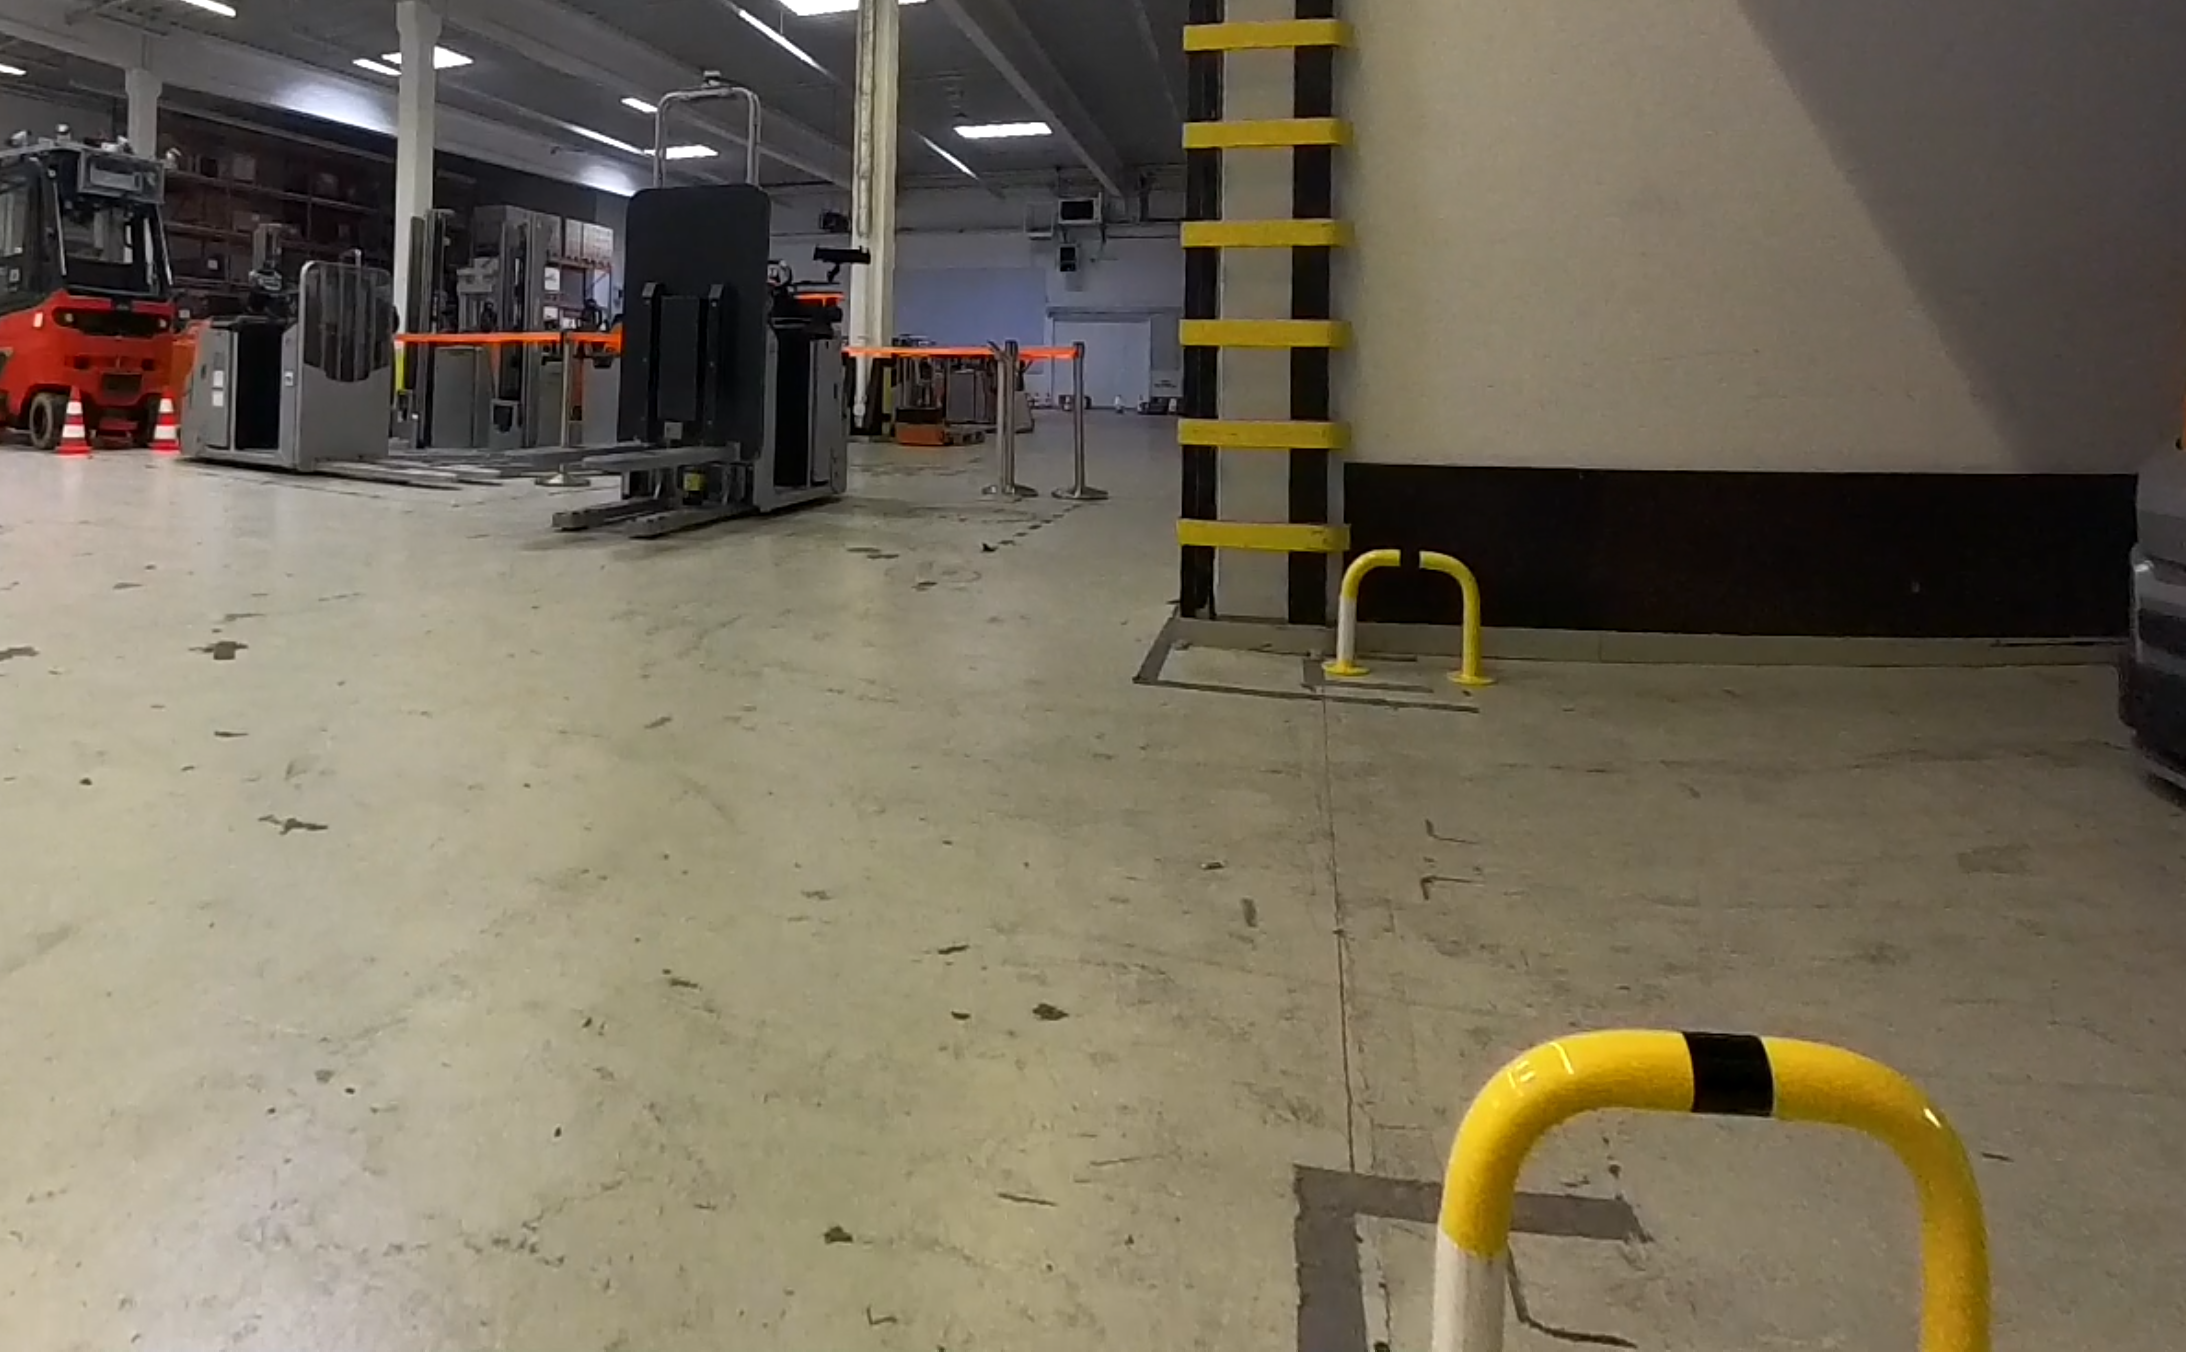
\includegraphics[width=5in]{images/Chap3/Test1_real_transition.png} % Replace with your figure
        \caption{Real Truck navigating the planned path: Transition phase}
        \label{OptResult51}
        \end{center}    
\end{figure}

The Truck follows the planned path and successfully 
transitions in the transition area while changing direction to orient the 
fork to the target.

\begin{figure}[H]
    \begin{center}
        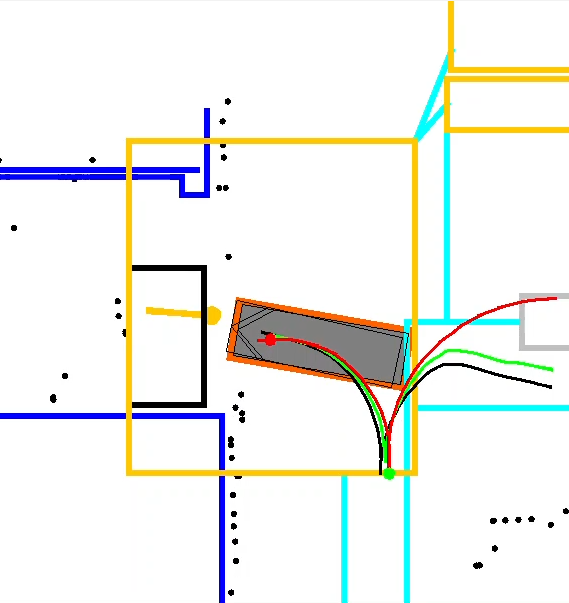
\includegraphics[width=3in]{images/Chap3/Test1_dock.png} % Replace with your figure
        \caption{Truck in the simulation navigating the planned path: Docking phase}
        \label{OptResult60}
        \end{center}    
\end{figure}


\begin{figure}[H]
    \begin{center}
        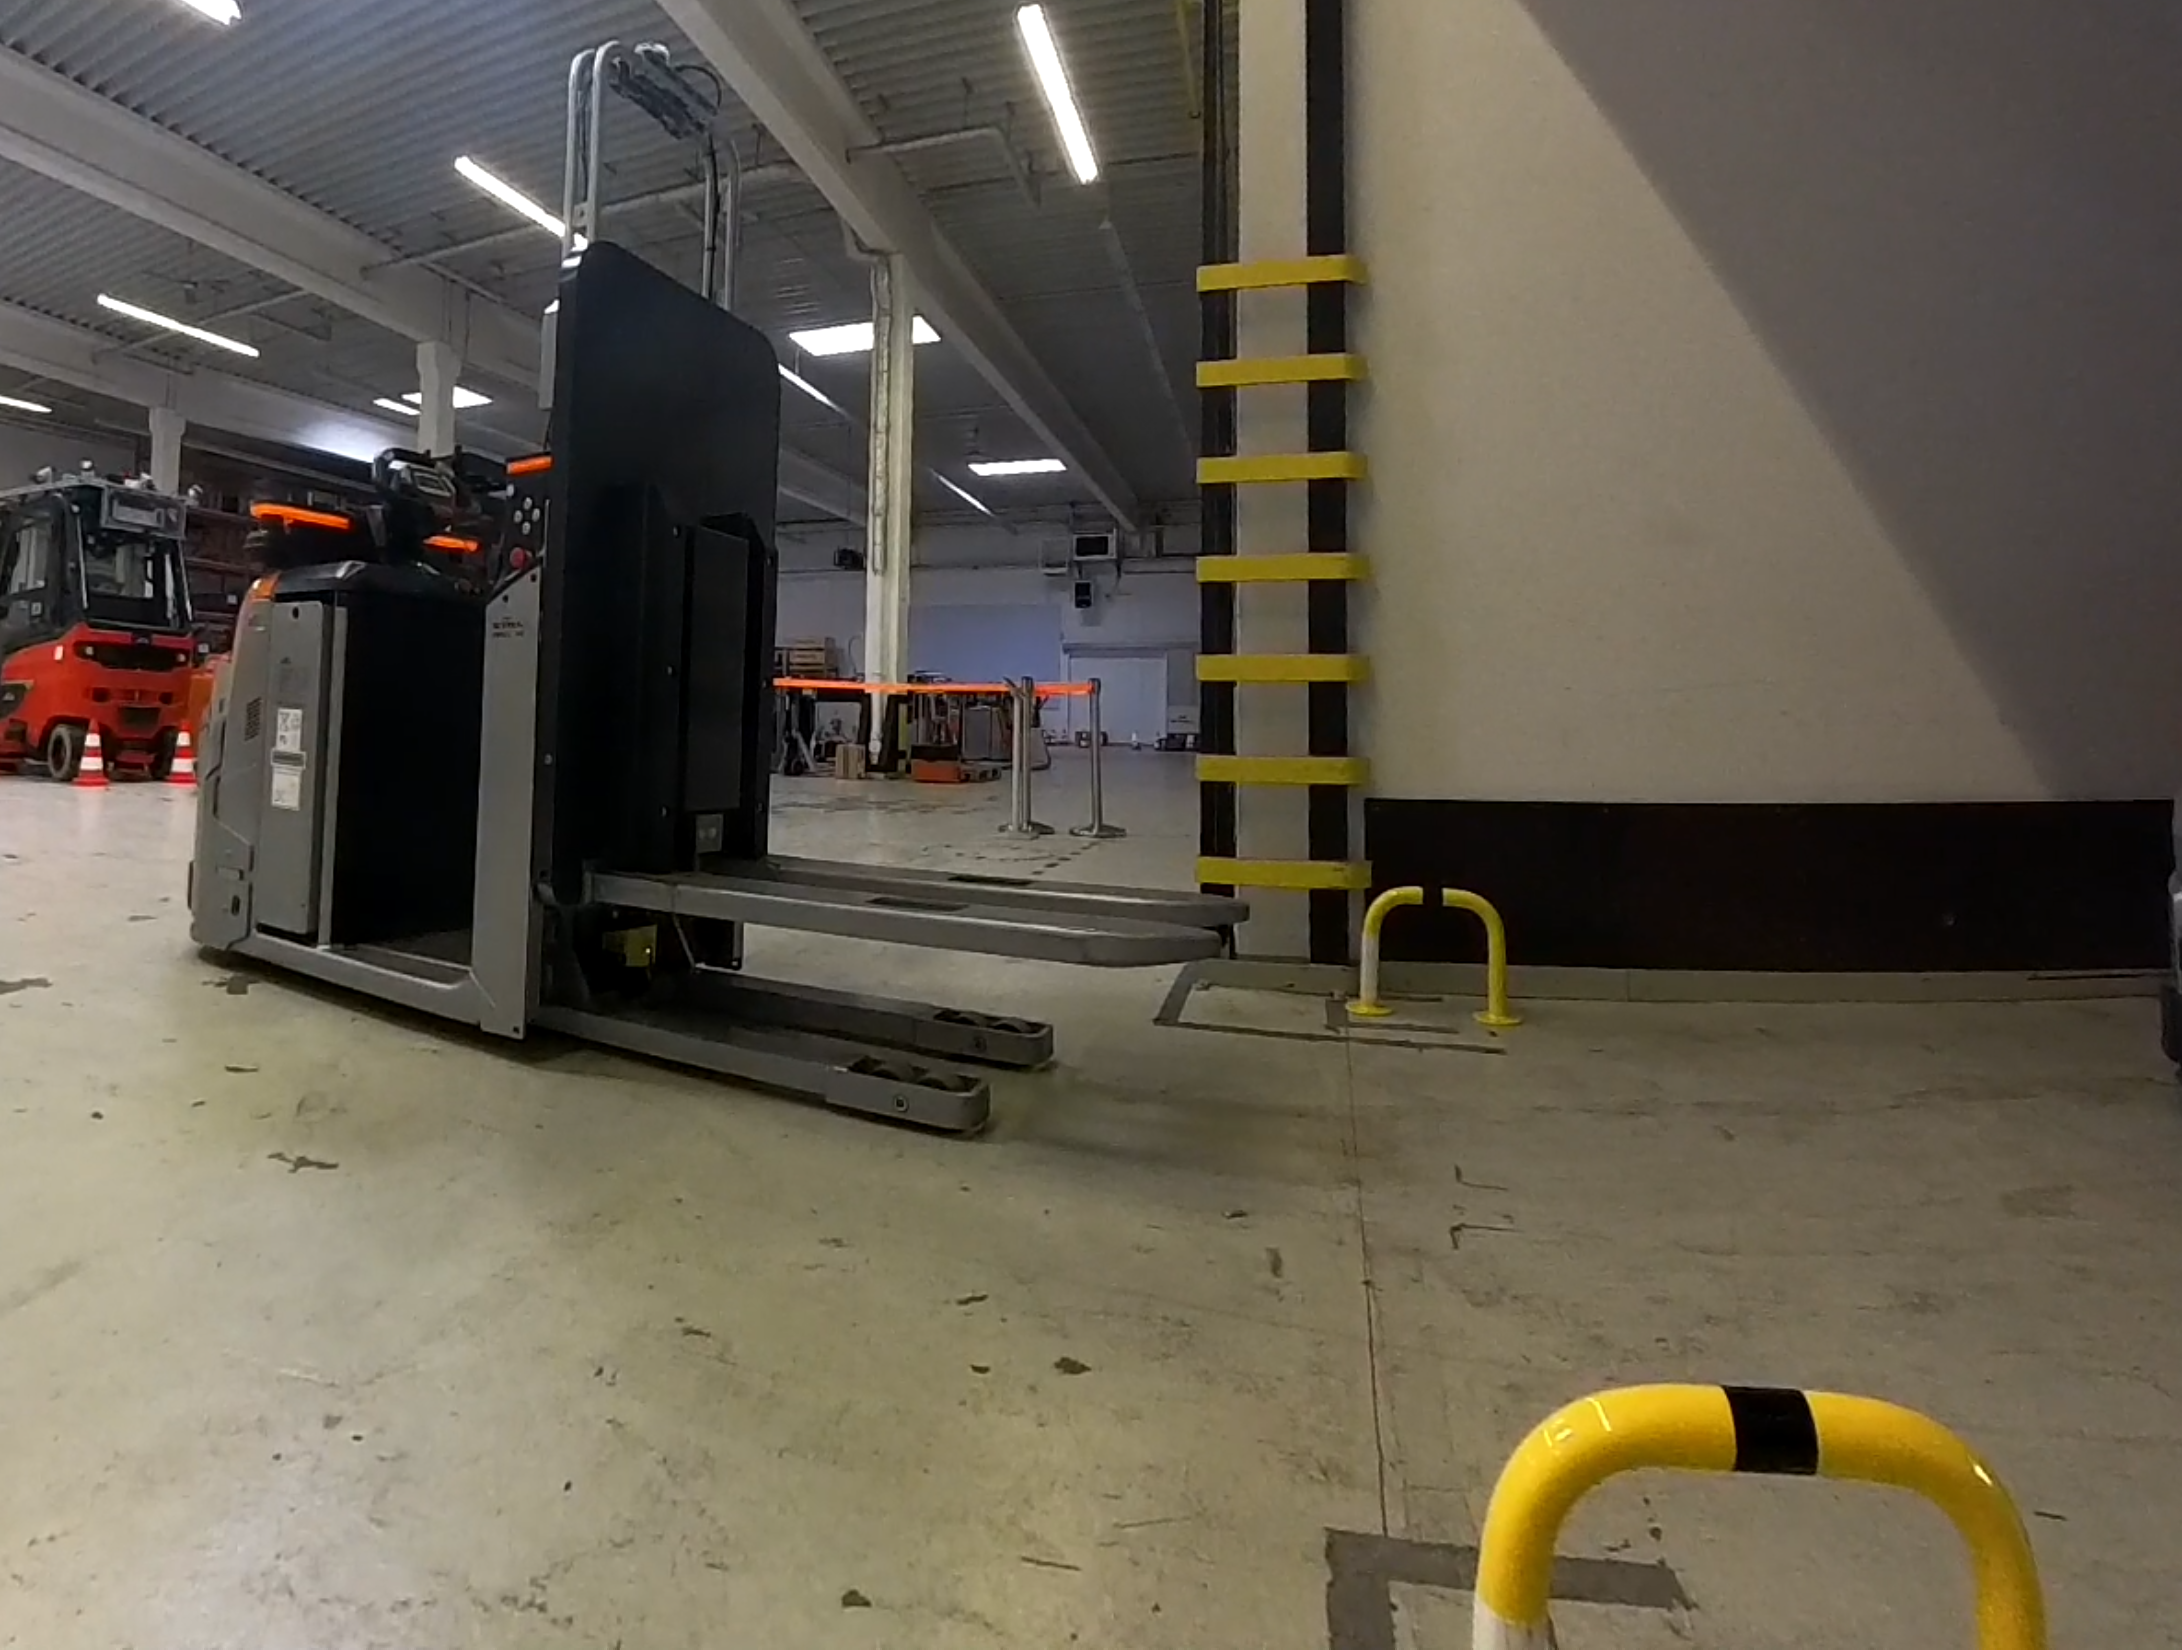
\includegraphics[width=4in]{images/Chap3/Test1_real_dock.png} % Replace with your figure
        \caption{Real Truck navigating the planned path: Docking phase}
        \label{OptResult61}
        \end{center}    
\end{figure}

The Truck arrives at the planned target and successfully 
docks the shelf with forks oriented towards it in preparation for
pickup / drop.

To summarize, for the test on the AMR, the PSO Algorithm is used. The duration of Planning of the optimized 
path was \(286ms\). 



\subsection{Complex Test Environments}
The Field-Tests in Complex Environments are conducted by placing obstacles on two sides of the 
station. 
Two test cases were carried out using two obstacle setups: Placing obstacles to the AMR's left then right
as illustrate figures \Ref{OptResult12} and \Ref{OptResult18}. 
The goal is to block one of the Transition zones, in order to test the system's flexibility,
exploration and exploitation of the transition possibilities.



\subsubsection{Obstacle Setup 1: Obstacle on the left of the AMR}

The truck was placed at position \(x = 33785\), \(y = 28845\), and \(\rho = 90.0^\circ\) as illustrated by figure 
\Ref{OptResult13}. The target is set at position \(x = 33356\), \(y = 22699\), and \(\rho = 270.0^\circ\).
The obstacle is as represented by figure \Ref{OptResult12}, a two-box block set one above the other. 
This obstacle was scanned and represented on the RACK Simulation 
Environment by its corner marked by the green arrow as illustrated by figure \Ref{OptResult13}.
The black dots seen on the same figure are scan points that represent obstacles in the warehouse. 
Usually there is more scan points, that cover for example the visible surface of an object.
For instance, the obstacle represented in figure \Ref{OptResult9} has scan points on its front side.
In the case illustrated by figure \Ref{OptResult13}, the scan points are reduced by using a RACK module 
that minimizes scan points concentrated in one area. The goal is to keep the necessary data about the surrounding 
objects and limit the amount of information to be processed 
for collision checking and path generation, thus optimizing processing time.
The optimum path is planned and the optimizer generates a pattern-based trajectory that transitions
inside the empty Transition Subpolygon. 
The generated path is illustrated in red on figure \Ref{OptResult15}. It is followed 
by the truck from the start, passing by the transition area and changing directions, and docking the 
target at the assigned position as represented on figure \Ref{OptResult16}. 

For this test setup, the planning duration of an optimum path is of \(303ms\). During this time
the optimizer processed a path that optimizes to a certain extent the path length and 
the curvature change proportionally to the path length.


\begin{figure}[H]
    \begin{center}
        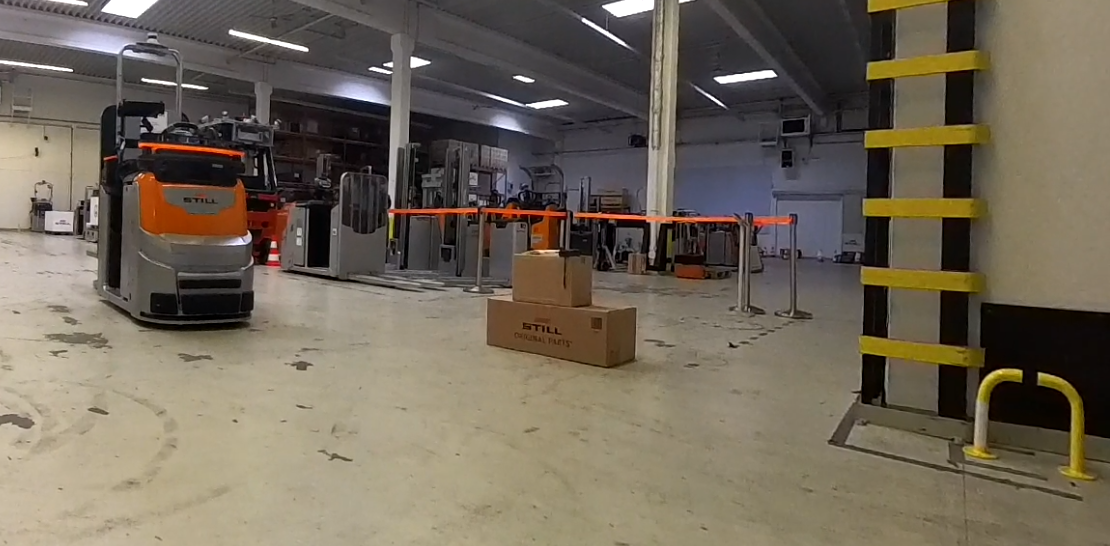
\includegraphics[width=5in]{images/Chap3/Test2_ObsLeftVehic/Start_real.png} % Replace with your figure
        \caption{Environment and Start position of the Complex Test Scenario: First Obstacle setup in the warehouse}
        \label{OptResult12}
        \end{center}    
\end{figure}

\begin{figure}[H]
    \begin{center}
        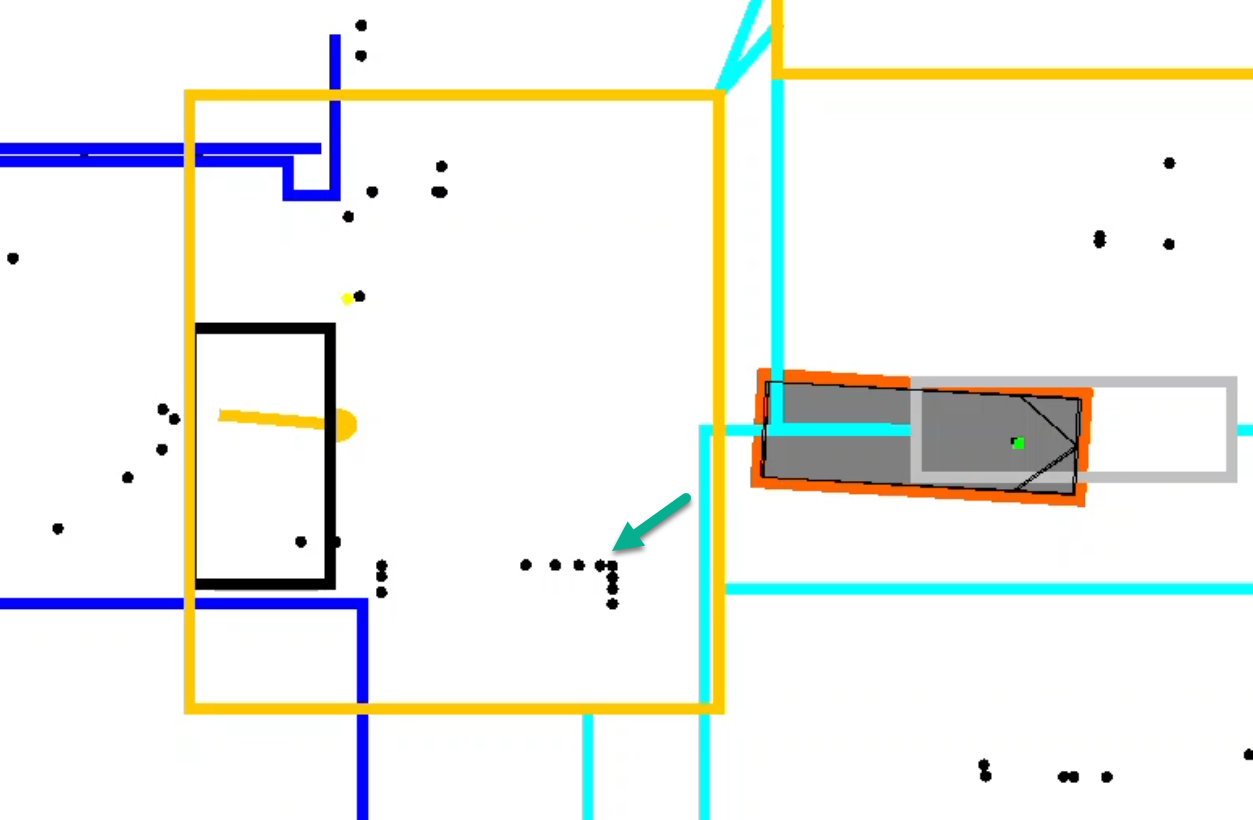
\includegraphics[width=4in]{images/Chap3/Test2_ObsLeftVehic/Start_simu.png} % Replace with your figure
        \caption{Environment and Start position of the Complex Test Scenario: First Obstacle setup in the simulation}
        \label{OptResult13}
        \end{center}    
\end{figure}

\begin{figure}[H]
    \begin{center}
        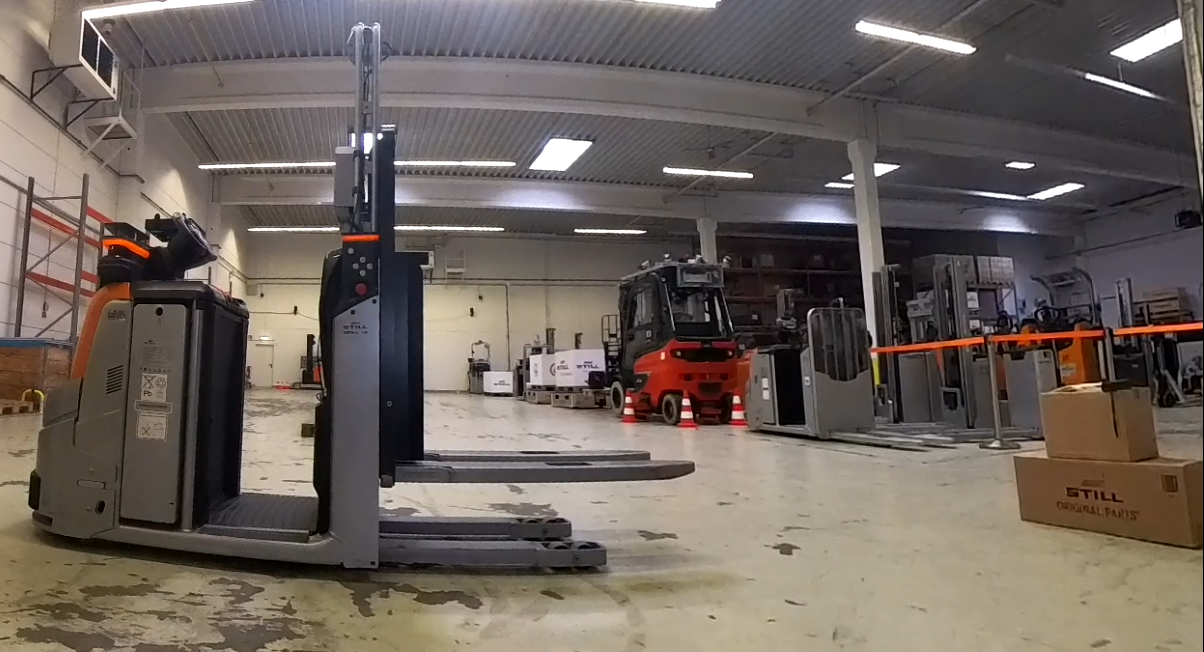
\includegraphics[width=5in]{images/Chap3/Test2_ObsLeftVehic/Transition_real.png} % Replace with your figure
        \caption{Transition Position of the Complex Test Scenario: First Obstacle setup in the warehouse}
        \label{OptResult14}
        \end{center}    
\end{figure}

\begin{figure}[H]
    \begin{center}
        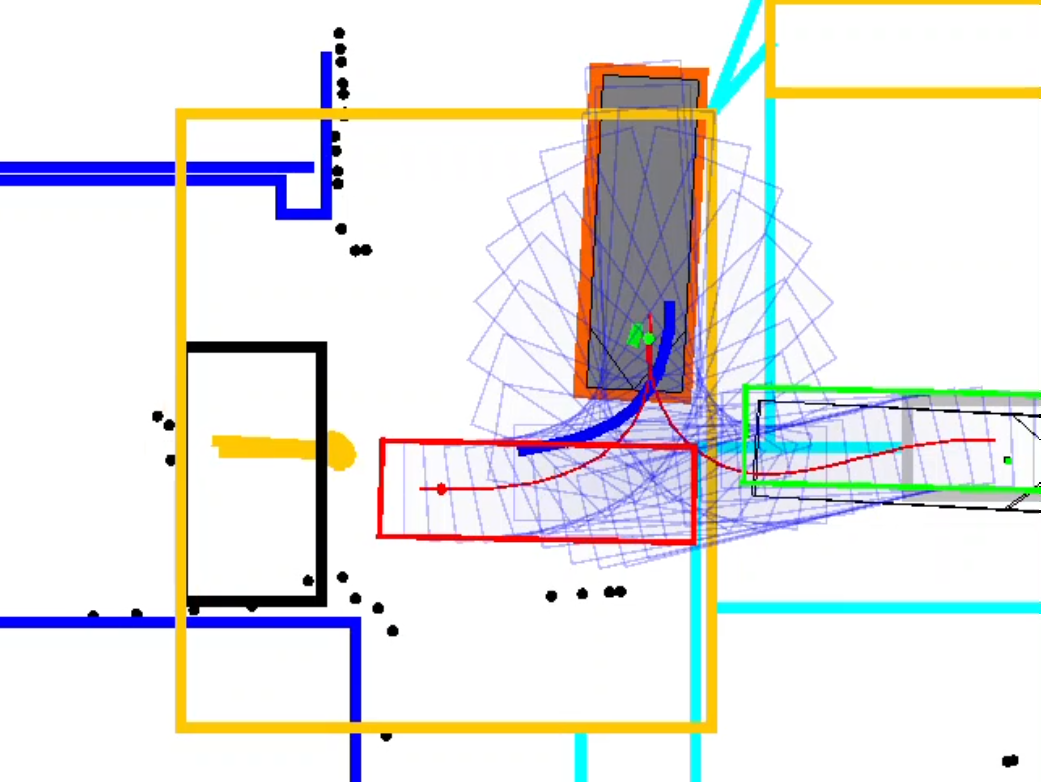
\includegraphics[width=4.5in]{images/Chap3/Test2_ObsLeftVehic/Transition_simu.png} % Replace with your figure
        \caption{Transition Position of the Complex Test Scenario: First Obstacle setup in the simulation}
        \label{OptResult15}
        \end{center}    
\end{figure}

\begin{figure}[H]
    \begin{center}
        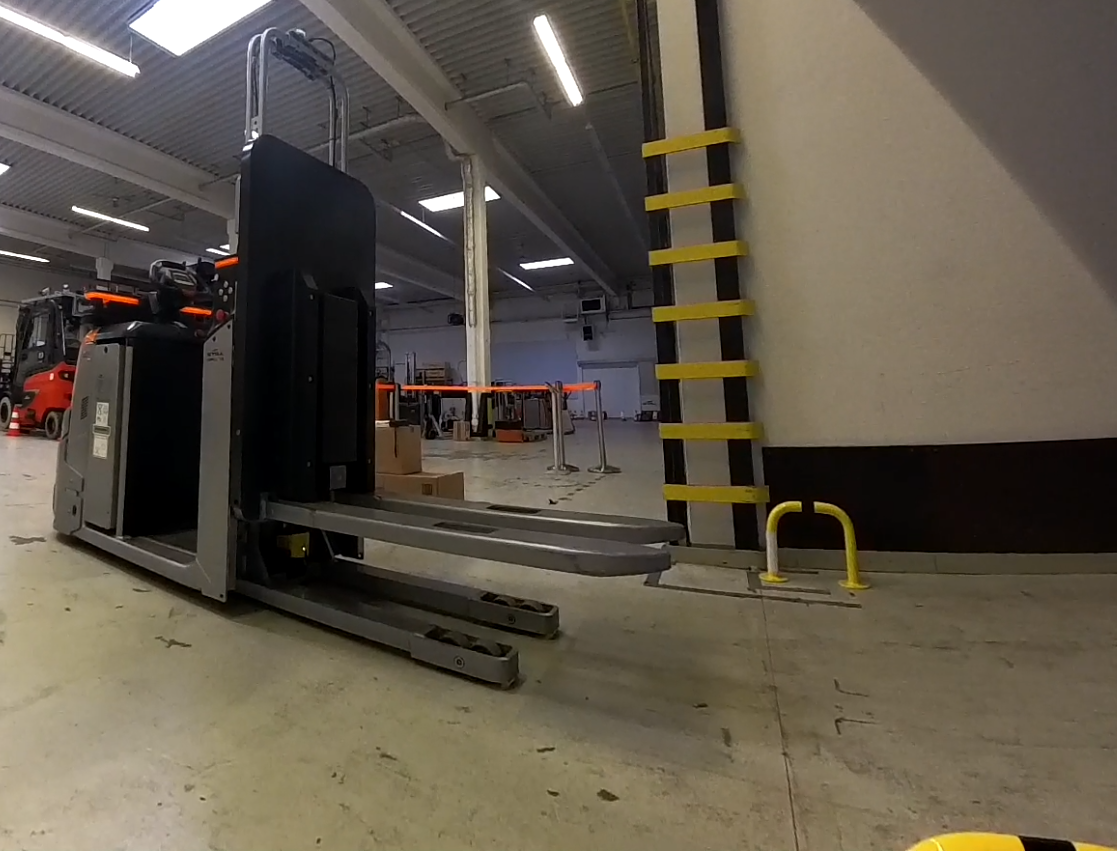
\includegraphics[width=4in]{images/Chap3/Test2_ObsLeftVehic/Target_real.png} % Replace with your figure
        \caption{Target Position of the Complex Test Scenario: First Obstacle setup in the warehouse}
        \label{OptResult16}
        \end{center}    
\end{figure}

\begin{figure}[H]
    \begin{center}
        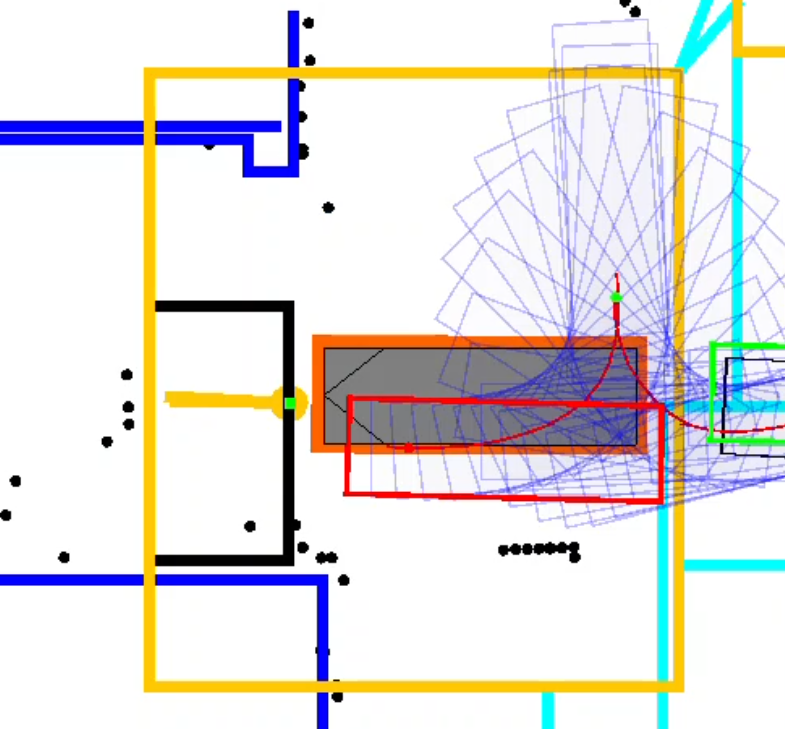
\includegraphics[width=4in]{images/Chap3/Test2_ObsLeftVehic/Target_simu.png} % Replace with your figure
        \caption{Target Position of the Complex Test Scenario: First Obstacle setup in the simulation}
        \label{OptResult17}
        \end{center}    
\end{figure}

\subsubsection{Obstacle Setup 2: Obstacle on the right of the AMR}

The truck was placed at position \(x =33891 \), \(y = 27760\), and \(\rho = 90.0^\circ\) as illustrated by figure 
\Ref{OptResult19}. The target is set at position \(x = 33492\), \(y = 22692\), and \(\rho = 270.0^\circ\).
The obstacle is a box represented by figure \Ref{OptResult18}. 
This obstacle was scanned and represented on the RACK Simulation 
Environment by its corner marked by the green arrow as illustrated by figure \Ref{OptResult19}.
The optimum path is planned and the optimizer generates a pattern-based trajectory that transitions
inside the empty Transition Subpolygon. 
The generated path is illustrated in red on figure \Ref{OptResult21}. It is followed 
by the truck from the start, passing by the transition area and changing directions, and docking the 
target at the assigned position as represented on figures \Ref{OptResult22} and \Ref{OptResult23}. 

For this test setup, the planning duration of an optimum path is of \(295ms\). During this time
the optimizer processed a path that optimizes to a certain extent the path length and 
the curvature change proportionally to the path length.

\begin{figure}[H]
    \begin{center}
        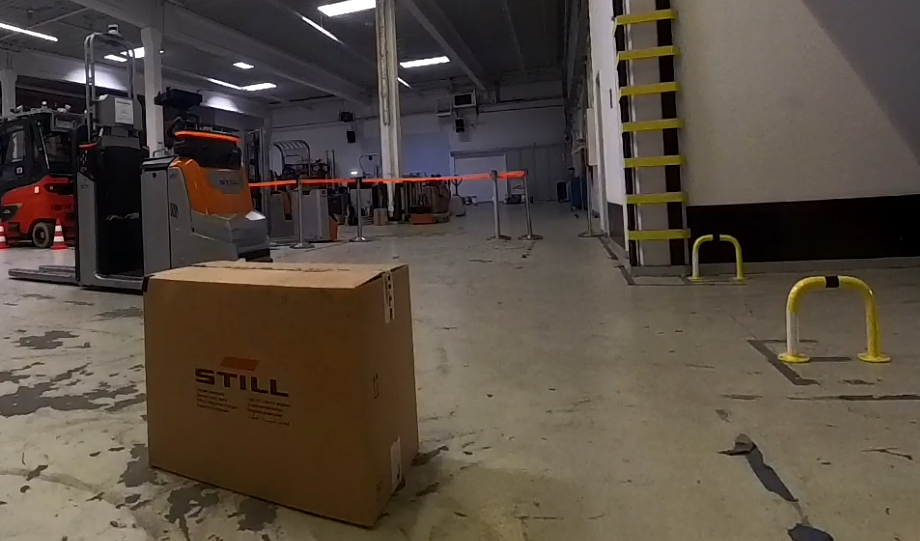
\includegraphics[width=4in]{images/Chap3/Test3/Start_real.png} % Replace with your figure
        \caption{Start Position of the Complex Test Scenario: Second Obstacle setup in the warehouse}
        \label{OptResult18}
        \end{center}    
\end{figure}

\begin{figure}[H]
    \begin{center}
        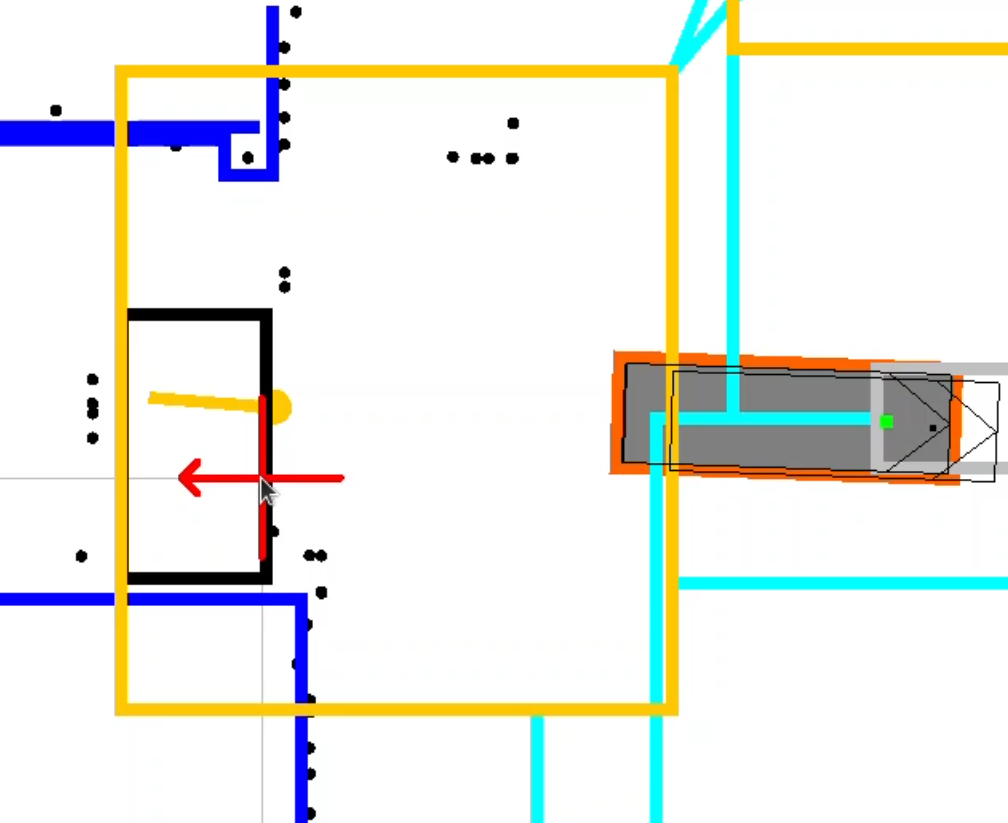
\includegraphics[width=4in]{images/Chap3/Test3/Start_simu.png} % Replace with your figure
        \caption{Start Position of the Complex Test Scenario: Second Obstacle setup in the simulation}
        \label{OptResult19}
        \end{center}    
\end{figure}

\begin{figure}[H]
    \begin{center}
        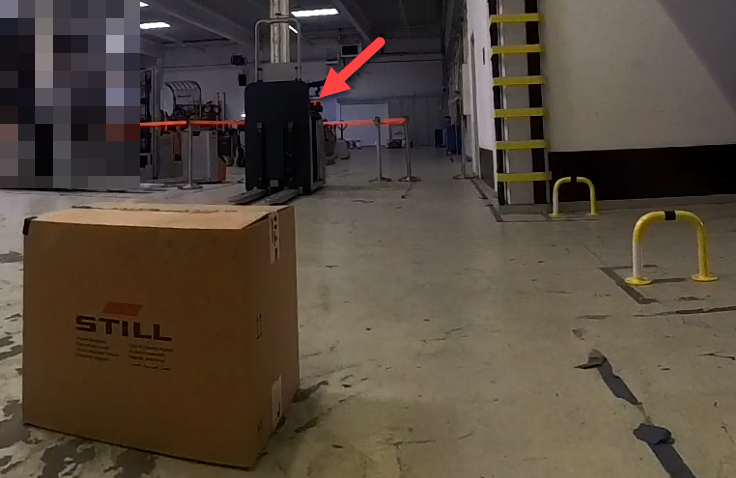
\includegraphics[width=4in]{images/Chap3/Test3/Transition_real.png} % Replace with your figure
        \caption{Transition Position of the Complex Test Scenario: Second Obstacle setup in the warehouse}
        \label{OptResult20}
        \end{center}    
\end{figure}

\begin{figure}[H]
    \begin{center}
        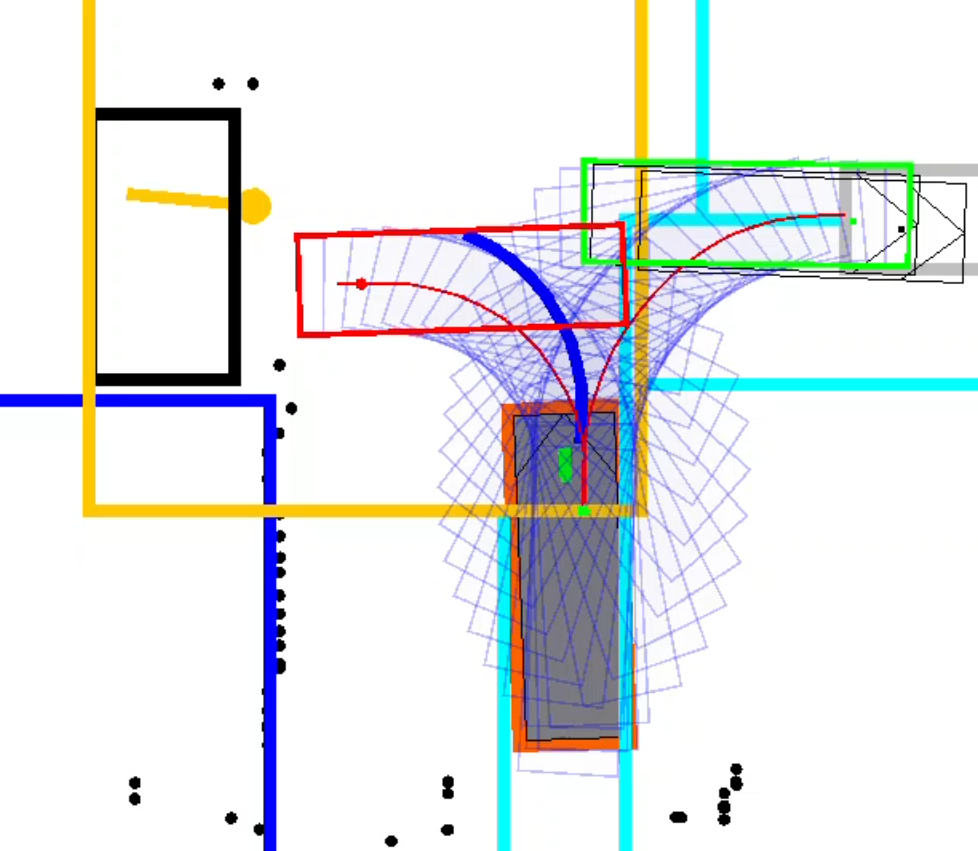
\includegraphics[width=4in]{images/Chap3/Test3/Transition_simu.png} % Replace with your figure
        \caption{Transition Position of the Complex Test Scenario: Second Obstacle setup in the simulation}
        \label{OptResult21}
        \end{center}    
\end{figure}

\begin{figure}[H]
    \begin{center}
        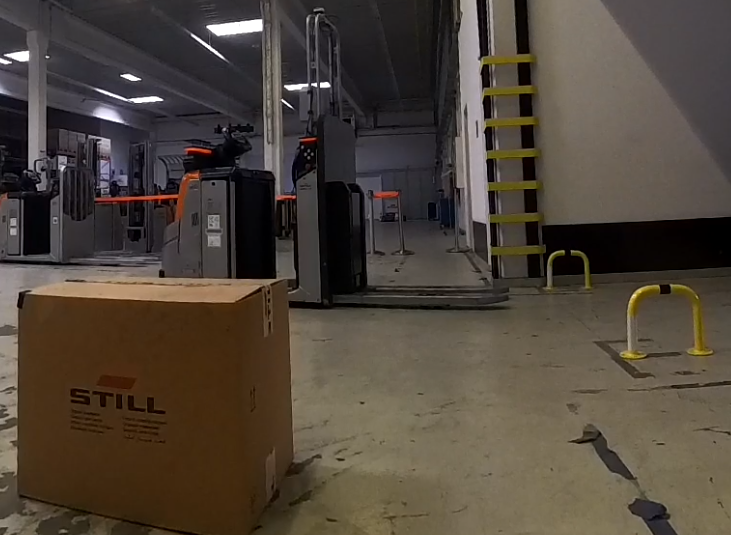
\includegraphics[width=4in]{images/Chap3/Test3/Target_Real.png} % Replace with your figure
        \caption{Target Position of the Complex Test Scenario: Second Obstacle setup in the warehouse}
        \label{OptResult22}
        \end{center}    
\end{figure}

\begin{figure}[H]
    \begin{center}
        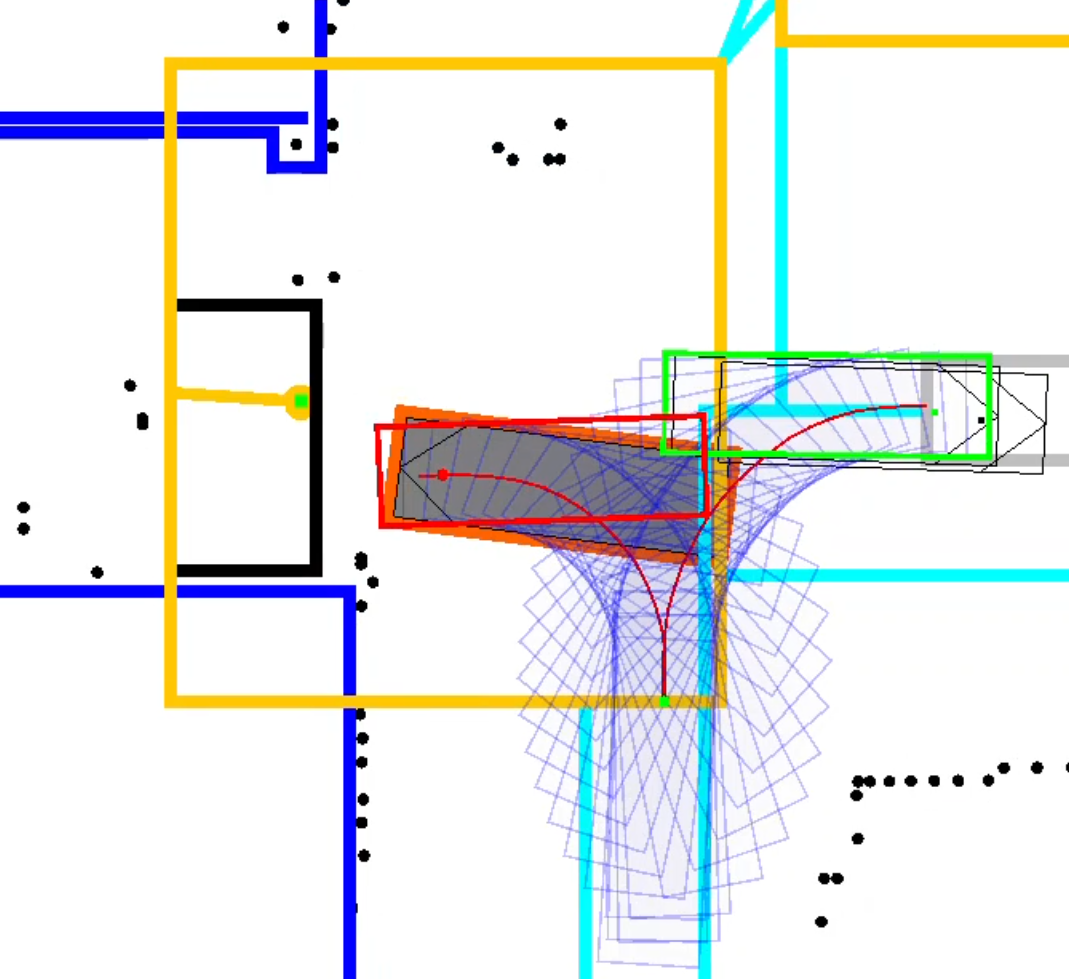
\includegraphics[width=4in]{images/Chap3/Test3/Target_simu.png} % Replace with your figure
        \caption{Target Position of the Complex Test Scenario: Second Obstacle setup in the simulation}
        \label{OptResult23}
        \end{center}    
\end{figure}



\subsection{Discussion of the results}

The Pattern-based path planning approach was tested in 3 different scenarios.
The PSO Algorithm was used for the 3 scenarios and successfully generated feasible paths for each 
test case. In the cases where obstacles were presented to the station the optimizer 
showcased the obstacle avoidance feature by rejecting colliding paths and opting for optimum
candidates that scored the least fitness values among the 200 generated individuals.
The previous test cases and events proved that the proposed approach is a simple and feasible 
solution to the docking process.
While the planning time in the RACK Simulation Environment was as low as \(59ms\) for the Simple Environment
and \(67ms\) for the Complex Environment, the field-testing scenarios scored planning times of 
\(286ms\) up to \(303ms\). 
This duration is significantly higher than the duration 
on the simulation. This is due to the high number of objects surrounding the vehicle which are 
represented by scan points that the truck needs to check for collisions for every path candidate.  
The traveled path can be shorter: the used Evaluation approach favors the optimization of the 
curvature term over the length, in other words, a longer path is better than a curved path.
This minimizes the curvature but creates long paths that have room for improvement. 

\section{Summary of Contributions and Reflections}
The goals set out for this thesis have been successfully achieved. A solution was developed that generates 
repeatable paths adhering to a predefined pattern, ensuring compliance with the specific layout and dimensions 
of the destination station. The solution is station-related, meaning it is tailored to the available space and 
dimensions of each station, allowing for precise accuracy in docking. Paths are generated within the goal's 
frame of reference, ensuring precision upon arrival. Additionally, optimization was achieved by focusing on 
both path length and curvature, utilizing metaheuristic algorithms to avoid obstacles while aligning with the 
kinematic constraints of the vehicle. This ensures an optimal and efficient route while respecting the physical 
limitations of the truck.

Several key gaps found in the literature, particularly related to intensive computational demands and long 
processing times in existing mobile robot path planning methods, have been addressed. The developed approach 
significantly reduces planning time, achieving times between 40 and 50 milliseconds in simulation and around 
300 milliseconds in field tests. In contrast, planning times in the literature range from 13 to 31 seconds 
(as outlined in Chapter 2, Section 4). Real-world challenges were addressed by simulating real obstacles and 
incorporating them into field tests. The pattern-based path generation approach also complies with the vehicle's 
kinematic constraints, such as turning radius, by limiting curvature, which ensures both computational efficiency 
and practical applicability in real-world scenarios.

The solution also fulfills the initial motivations by providing explainable and predictable paths. Maneuvering 
and direction changes are clearly interpretable by human operators, ensuring transparency in the system’s behavior. 
The decision-making process is also explainable, with the optimizer’s parameters—path length and curvature—clearly 
defined and weighted. The ease of commissioning is preserved, as the system is designed to recognize stations 
easily and is adaptable to any station, regardless of its orientation (as demonstrated in the tests conducted on 
two stations in Chapter 4). By addressing these key points, the solution enhances customer trust and confidence 
while maintaining both autonomy and operational efficiency.

\subsection*{Conclusion}
In this chapter, the proposed solution was rigorously tested and validated through a series of evaluations, 
beginning with path creation and extending to path optimization and real-world field-testing. 
The results demonstrated the effectiveness of the solution in creating, evaluating, and optimizing paths, 
with each stage providing valuable insights into its performance. The field tests conducted in a simple 
environment using an Autonomous Mobile Robot (AMR) confirmed that the proposed solution could be effectively 
deployed in practical scenarios. The discussion highlighted key takeaways, underscoring the robustness 
and applicability of the solution in real-world settings.